\documentclass[journal=asbcd6,manuscript=article]{achemso}

\usepackage{natbib}
\usepackage{setspace}
\usepackage{xkeyval}
\usepackage{array}
\usepackage{listings}
\usepackage{lmodern}
\usepackage{mathpazo}
\usepackage{geometry}
\usepackage{microtype}
\usepackage{url}  % Formatting web addresses
\usepackage{ifthen}  % Conditional
\usepackage{multicol}   %Columns
\usepackage[utf8]{inputenc} %unicode support
\usepackage{amsmath}
\usepackage{amssymb}
\usepackage{mathtools}
\usepackage{epsfig}
\usepackage{epstopdf}
\usepackage{graphicx}
\usepackage{textcomp}
\usepackage{multirow}
\usepackage{booktabs}
\usepackage{natmove}
\usepackage{float}
\usepackage[margin=0.1pt,font=footnotesize,labelfont=bf]{caption}
\usepackage[version=3]{mhchem} % Formula subscripts using \ce{}
\usepackage[T1]{fontenc}       % Use modern font encodings
%\usepackage[square,sort,comma,numbers,sort&compress]{natbib}
%%%%%%%%%%%%%%%%%%%%%%%%%%%%%%%%%%%%%%%%%%%%%%%%%%%%%%%%%%%%%%%%%%%%%
%% If issues arise when submitting your manuscript, you may want to
%% un-comment the next line.  This provides information on the
%% version of every file you have used.
%%%%%%%%%%%%%%%%%%%%%%%%%%%%%%%%%%%%%%%%%%%%%%%%%%%%%%%%%%%%%%%%%%%%%
%%\listfiles

%\bibliographystyle{achemso}
\newcommand*\mycommand[1]{\texttt{\emph{#1}}}
%%%%%%%%%%%%%%%%%%%%%%%%%%%%%%%%%%%%%%%%%%%%%%%%%%%%%%%%%%%%%%%%%%%%%

%%%%%%%%%%%%%%%%%%%%%%%%%%%%%%%%%%%%%%%%%%%%%%%%%%%%%%%%%%%%%%%%%%%%%
\author{Michael Vilkhovoy}
\affiliation[Cornell University]
{Robert Frederick Smith School of Chemical and Biomolecular Engineering, Cornell University, Ithaca, NY 14853}
\author{Nicholas Horvath}
\affiliation[Cornell University]
{Robert Frederick Smith School of Chemical and Biomolecular Engineering, Cornell University, Ithaca, NY 14853}
\author{Joseph Wayman}
\affiliation[Cornell University]
{Robert Frederick Smith School of Chemical and Biomolecular Engineering, Cornell University, Ithaca, NY 14853}
\author{Kara Calhoun}
\affiliation[Stanford University]
{School of Chemical Engineering, Stanford University, Stanford, CA 94305}
\author{James Swartz}
\affiliation[Stanford University]
{School of Chemical Engineering, Stanford University, Stanford, CA 94305}
\author{Jeffrey D. Varner}
\email{jdv27@cornell.edu}
\phone{+1~(607)~255-4258}
\fax{+1~(607)~255-9166}
\affiliation[Cornell University]
{Robert Frederick Smith School of Chemical and Biomolecular Engineering, Cornell University, Ithaca, NY 14853}
%%%%%%%%%%%%%%%%%%%%%%%%%%%%%%%%%%%%%%%%%%%%%%%%%%%%%%%%%%%%%%%%%%%%%
\title{Sequence Specific Modeling of Cell-Free Protein Synthesis}
%\abbreviations{MV,NH,JDV}
\keywords{Synthetic biology, constraints based modeling, cell-free protein synthesis}

\begin{document}

%%%%%%%%%%%%%%%%%%%%%%%%%%%%%%%%%%%%%%%%%%%%%%%%%%%%%%%%%%%%%%%%%%%%%
%% The abstract environment will automatically gobble the contents
%% if an abstract is not used by the target journal.
%%%%%%%%%%%%%%%%%%%%%%%%%%%%%%%%%%%%%%%%%%%%%%%%%%%%%%%%%%%%%%%%%%%%%
\begin{abstract}
In this study, we used sequence specific constraints based modeling to evaluate the performance of synthetic circuits in an \emph{E.~coli} cell-free protein synthesis system.
A core \emph{E.~coli} metabolic model, consisting of glycolysis, pentose phosphate pathway, amino acid biosynthesis and degradation and energy metabolism, was then augmented with sequence specific descriptions of genetic circuits which included mechanistic models of promoter function, transcription and translation.
Thus, unlike other synthetic biology modeling efforts, sequence specific constraints based modeling explicitly couples the transcription and translation of circuit components with the availability of metabolic resources.
Model parameters for transcription and translation were taken from literature, allowing a first principles prediction of circuit performance.
We tested this approach by first simulating T7 induced chloramphenicol acetyltransferase production and P70a-induced deGFP expression; we then expanded these studies for a range of different proteins.
First principles predictions of circuit performance were consistent with measurements for a variety of cases.
Further, global sensitivity analysis identified the key metabolic processes that controlled circuit performance in terms of productivity, energy efficiency, and carbon yield.
A sufficient energy supply with oxidative phosphorylation is instrumental for high energy efficiency and carbon yields; in addition, the translation rate could be optimized for higher productivity.
Taken together, sequence specific constraints based modeling offers a novel means to \emph{a~priori} estimate the performance of cell-free synthetic circuits.
\end{abstract}

%%%%%%%%%%%%%%%%%%%%%%%%%%%%%%%%%%%%%%%%%%%%%%%%%%%%%%%%%%%%%%%%%%%%%
%% Start the main part of the manuscript here.
%%%%%%%%%%%%%%%%%%%%%%%%%%%%%%%%%%%%%%%%%%%%%%%%%%%%%%%%%%%%%%%%%%%%%

\section{Introduction}
Cell-free protein expression has become a widely used research tool in systems and synthetic biology, and a promising technology for personalized protein production.
Cell-free systems offer many advantages for the study, manipulation and modeling of metabolism compared to \textit{in vivo} processes.
Central amongst these, is direct access to metabolites and the biosynthetic machinery without the interference of a cell wall, or complications associated with cell growth.
This allows us to interrogate the chemical environment while the biosynthetic machinery is operating, potentially at a fine time resolution.
Cell-free protein synthesis (CFPS) systems are arguably the most prominent examples of cell-free systems used today \cite{Jewett:2008aa}.
However, CFPS is not new; CFPS in crude \textit{E.~coli} extracts has been used since the 1960s to explore fundamental biological mechanisms \cite{MATTHAEI:1961aa,NIRENBERG:1961aa}.
Today, cell-free systems are used in a variety of applications ranging from therapeutic protein production \cite{Lu:2014aa} to synthetic biology \cite{Hodgman:2012aa}.
However, if CFPS is to become a mainstream technology for applications such as point of care manufacturing, we must first understand the performance limits of these systems.
One tool to address this question is mathematical modeling.

% Interestingly, many of the challenges confronting \textit{in~vivo} genome scale kinetic modeling can potentially be overcome in a cell-free system.
% For example, there is no complex transcriptional regulation to consider, transient metabolic measurements are easier to obtain, and we no longer have to consider cell growth.
% Thus, cell-free operation holds several significant advantages for model development, identification and validation.
% Theoretically, genome scale cell-free kinetic models may be possible for industrially important organisms, such as \textit{E.~coli} or \textit{B. subtilis}, if a simple, tractable framework for integrating allosteric regulation with enzyme kinetics can be formulated.
% Traditionally, stoichiometric models have also neglected explicit descriptions of metabolic regulation and control mechanisms, instead opting to describe the choice of pathways by prescribing an objective function on metabolism. Interestingly, similar to early cybernetic models, the most common metabolic objective function has been the optimization of biomass formation \cite{2002_ibarra_edwards_palsson_Nat}, although other metabolic objectives have also been estimated \cite{2007_schuetz_sauer_MolSysBio}.
% Recent advances in constraints based modeling have overcome the early shortcomings of the platform, including capturing metabolic regulation and control \cite{2013_hyduke_lewis_palsson_MolBioSys}. Thus, modern constraints based approaches are extremely useful for the discovery of metabolic engineering strategies and represent the state of the art in metabolic modeling \cite{2013_mccloskey_palsson_feist_MolSysBio, 2012_zomorrodi_maranas_MetaEng}.

Stoichiometric reconstructions of microbial metabolism, popularized by flux balance analysis (FBA), have become standard tools to interrogate metabolism \cite{2012_lewis_palsson_NatRevMicrobio}.
Since the first genome scale stoichiometric model of \textit{E.~coli} \cite{2000_edwards_palsson_PNAS}, stoichiometric reconstructions of hundreds of organisms, including industrially important prokaryotes such as \textit{E.~coli} \cite{Feist:2007aa} or \textit{B. subtilis} \cite{Oh:2007aa}, are now available \cite{2009_feist_palsson_NatRevMicrobio}.
In this study, we used sequence specific constraints based modeling to evaluate the performance of \emph{E.~coli} cell-free protein synthesis (CFPS).
A core \emph{E.~coli} cell-free metabolic model was developed from literature \cite{Feist:2007aa}.
This model, which described glycolysis, pentose phosphate pathway, amino acid biosynthesis and degradation and energy metabolism, was then augmented with
sequence specific descriptions of promoter function, transcription and translation processes.
Thus, sequence specific constraints based modeling explicitly coupled transcription and translation with the availability of metabolic resources.
We tested this approach by simulating the production of two model proteins, and then investigated the productivity, energy efficiency, and carbon yield for eight different proteins.
From this, higher carbon number proteins typically had lower productivity rates, energy efficiency, and carbon yields than that of the lower carbon number proteins.
Further, global sensitivity analysis identified the key metabolic processes that controlled circuit performance, showing oxidative phosphorylation as instrumental for maintaining a high energy efficiency and carbon yield and the translation rate for productivity.
Taken together, sequence specific constraints based modeling offers a novel means to \emph{a~priori} estimate the performance of cell-free synthetic circuits.

\clearpage

\section{Results and discussion}


% The goal of this work was first to construct a modeling framework to describe cell-free protein synthesis systems and to examine its performance in productivity, energy efficiency and carbon yield for a protein of interest.
% One mathematical framework that has found wide use in modeling metabolism is constraints based models such as flux balance analysis (FBA).
% FBA can predict how cells utilize nutrients to produce products by using the biochemical stoichiometry and thermodynamical feasibility under pseudo steady-state conditions.
% Traditionally, FBA is used to model \textit{in~vivo} processes; however, cell-free systems do not have growth associated reactions or transport through the cell membrane.
% Thus,
% sequence specific flux balance analysis (ssFBA) with a detailed promoter model  to examine the performance of CFPS.
% We first validated the ssFBA approach by comparing simulated and measured concentrations of two proteins from two

\subsection{Model derivation and validation}
The cell-free stoichiometric network was constructed by removing growth associated reactions from the \textit{i}AF1260 reconstruction of K-12 MG1655 \textit{E.~coli} \cite{Feist:2007aa}.
We then added the transcription and translation template reactions of Allen and Palsson for the specific proteins of interest \cite{Allen:2003aa}.
A schematic of the metabolic network, which consisted of 264 reactions and 146 species, is shown in Fig.~\ref{fig:network}A.
Using this network, in combination with detailed promoter models, and literature values for cell-free culture parameters (Table ~\ref{tbl:parameters}),
we simulated the sequence specific production of two model proteins, chloramphenicol acetyltransferase (CAT) and dual emission green fluorescent protein (deGFP) using
different cell-free \textit{E.~coli} extracts. The cell-free metabolic network, model parameters, model code,
and each protein sequence are available in the supplemental materials.

Cell-free simulations predicted CAT and deGFP production for the duration of the CFPS batch reactions (Fig. ~\ref{fig:network}B and C).
Chloramphenicol acetyltransferase (CAT), was produced under a T7 promoter in a glucose/NMP cell-free system \cite{2005_calhoun_BiotechnologyProgress} for 1 hour using glucose as a carbon and energy source (Fig.~\ref{fig:network}B).
With the exception of the first 10-15 min, the cell-free prediction of CAT abundance was consistent with the measured values.
On the other hand, deGFP was produced under a P70a promoter in TXTL 2.0 \textit{E.~coli} extract for 8 hours using maltose as a carbon and energy source (Fig.~\ref{fig:network}C).
The cell-free simulation captured the overall trend of deGFP abundance, but was not able to capture saturation at the end of the CFPS culture.
Uncertainty in experimental factors such as the concentration of RNA polymerase, ribosomes,
transcription and translation elongation rates and the upper bounds for oxygen and glucose consumption rates did not alter the qualitative performance of the model.
Thus, the metabolic network and molecular description of transcription and translation were consistent with experimental measurements.
\begin{figure}[t!]
\centering
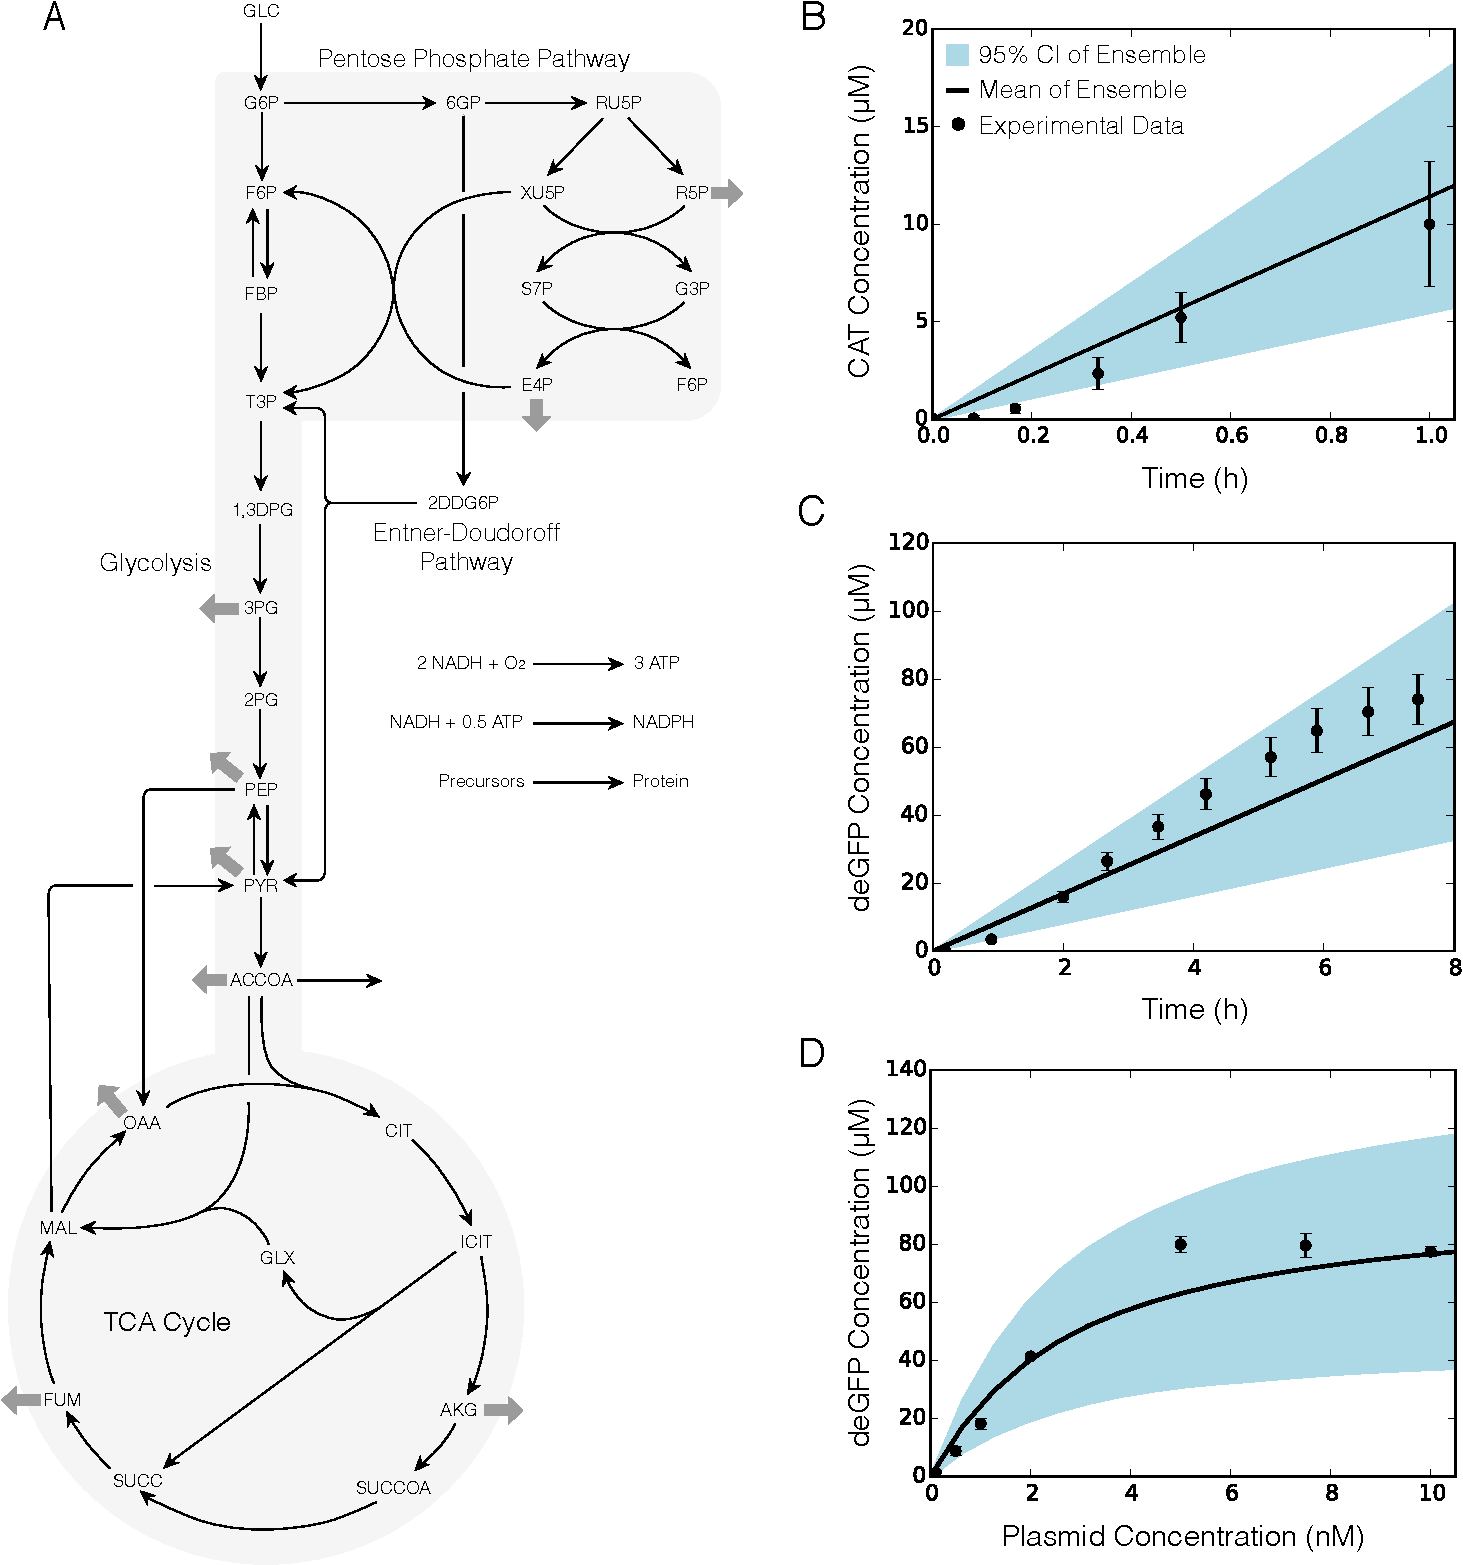
\includegraphics[width=1.00\textwidth]{./Figures/ssFBA_network.pdf}
\caption{Sequence specific flux balance analysis. A. Core metabolic network with glycolysis, pentose phoshate pathway, TCA cycle, Entner-Doudoroff pathway. Thick gray arrows indicate withdrawal of precursors for amino acid synthesis. B. CAT production under a T7 promoter in CFPS \textit{E.~coli} extract for 1 h under glucose consumption. Error bars denote the standard deviation of experimental measurements. C. deGFP production under a P70 promoter in TXTL 2.0 \textit{E.~coli} extract for 8 h under maltose consumption. Error bars denote a 10\% coefficient of variation. D. Predicted deGFP concentration at different plasmid concentrations versus measurements of deGFP synthesized in TXTL 2.0. 95\% CI (blue region) over the ensemble of 100 sets, mean of the ensemble (black line), and experimental measurements (dots).}
\label{fig:network}
\end{figure}

Next, we predicted deGFP production as a function of plasmid concentration (Fig.~\ref{fig:network}D).
Concentration of deGFP at each plasmid concentration was calculated by multiplying the flux of deGFP synthesis by the active time of production, approximately 8 hours in TXTL 2.0 \cite{Garamella:2016aa}.
The mean of the ensemble shows a good prediction against the measured deGFP levels, even though it under predicted deGFP concentration at the saturating point of 5 nM of plasmid concentration.
However, the ensemble and the mean of the ensemble captured the overall saturating dynamics of deGFP production as a function of plasmid concentration.
These results validated our mathematical framework to model CFPS systems and predict the production of two proteins with very few adjustable parameters.
It also showed that the sequence specific reactions were sufficient to predict the production of two different proteins under different promoters and cell-free systems.
Since the model accurately predicted protein production, we used our mathematical framework to understand the performance limits of CFPS.

\subsection{Analysis of CFPS performance}
Our next goal was to examine the performance of CFPS for eight different proteins under three different cases.
Each of the proteins was produced under a P70a promoter, except for CAT which was produced under a T7 promoter.
In all cases, CFPS was supplied with glucose.
In the first case, CFPS was supplied with amino acids, and the system was allowed to synthesize amino acids (AA uptake and synthesis).
In the second case, CFPS was supplied with amino acids, but the amino acid synthesis reactions were turned off (AA uptake w/o synthesis).
These amino acid synthesis reactions were blocked since during the cell-free extract preparation the cells are often supplied with amino acids; thus, the enzymes responsible for amino acid synthesis would not be present.
In the third case, CFPS was not supplied with amino acids, but the system could synthesize them (AA synthesis w/o uptake).
Eight different proteins, ranging in size, were selected to evaluate CFPS performance: bone morphogenetic protein 10 (BMP10), chloramphenicol acetyltransferase (CAT), caspase 9 (CASP9), dual emission green fluorescent protein (deGFP), prothrombin (FII), coagulation factor X (FX), fibroblast growth factor 21 (FGF21), and single chain variable fragment R4 (scFvR4).
We used ssFBA to estimate the productivity, energy efficiency, and carbon yield for each of these proteins for each case.
An additional case was considered for CAT, since a comprehensive dataset is available (Supporting Information); in this case, fluxes were constrained to experimental measurements where avaliable, with the exception of CAT production which was determined by the transcription/translation parameters.

\subsubsection{Productivity}
The mean productivity was inversely proportional to the protein size and varied between 1 and 12 $\mu$M/h for the proteins sampled (Fig.~\ref{fig:Prod}).
All cases had very similar performance for each protein and were within a standard deviation of each other (Fig.~\ref{fig:Prod}A).
%with the second case (without amino acid synthesis) having a slightly higher productivity for most proteins.
The model framework is setup to optimize for the production of each protein and is constrained by the translation rate.
This shows the system had sufficient substrates and metabolic precursors to power CFPS and synthesize each protein of interest with the same productivity, regardless of the case.
However, each individual protein had a different level of productivity.
For instance, BMP10 had a productivity of about 2.5 $\mu$M/h whereas CAT had a productivity of about 12 $\mu$M/h.
To examine this further, the mean productivity was plotted against the carbon number of each protein (Fig.~\ref{fig:Prod}B).
The proteins with the highest productivity had the lowest carbon number, whereas proteins with low productivity had higher carbon numbers.
This inverse trend was due to the fact that larger proteins require more amino acids and substrates to assemble them, resulting in lower productivity given the same resources.
A single trendline for all cases shows the expected productivity in CFPS depending on the carbon number of the protein of interest (available in the Supporting Information).
CAT was an outlier for the trendline, even though it was in the same order of magnitude as the trendline.
The relative high productivity of CAT was due to its T7 promoter.
CAT on a P70a promoter frollowed the same trendline as the other proteins and had a productivity of about 8.8 $\mu$M/h. 
Taken together, a single trendline showed good agreement (R\textsuperscript{2} = 0.99) with estimating the expected productivity of a protein on a P70a promoter in CFPS, given the size of the protein.
%The higher productivity of CAT compared to all other proteins was most likely due to the lower transcription requirement of cytidine triphosphate which allowed a higher flux for translation.
% further study on the nucleotide and amino acid requirements of each protein and its effect on CFPS performance should be investigated.
\begin{figure}[t!]
\centering
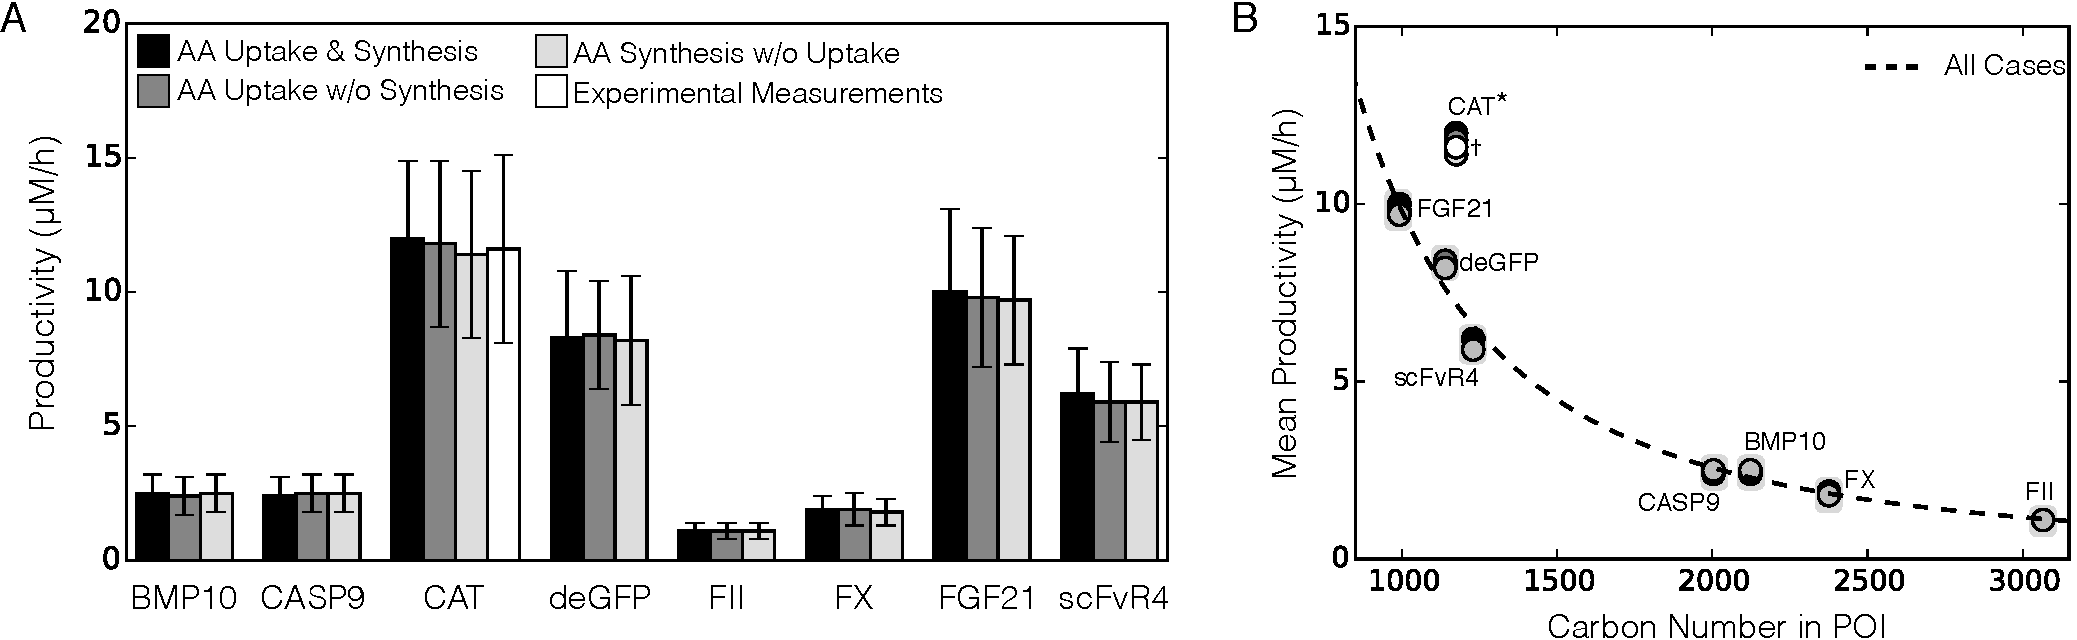
\includegraphics[width=1.00\textwidth]{./Figures/Productivity.pdf}
\caption{CFPS productivity of eight proteins for four cases. Amino acid uptake and synthesis (black), AA uptake without synthesis (dark grey), AA synthesis without uptake (light grey), and constrained by experimental measurements, for CAT only (white). A. Productivity across the ensemble (error bars represent 95\% CI). B. Mean productivity versus carbon number. Single trendline (dotted line) calculated across all cases (y = 6015004x\textsuperscript{-1.9}; R\textsuperscript{2} = 0.99). Asterisk: protein excluded from trendline; dagger: constrained by experimental measurements and excluded from trendline.}
\label{fig:Prod}
\end{figure}

\subsubsection{Energy efficiency}
The energy efficiency of protein production remained relatively high for when amino acids were supplied in the media, however energy efficiency dropped below 32\% when amino acids were not available (Fig.~\ref{fig:Energy}).
Following the same outline as in examining the productivity, we calculated the energy efficiency of production for each protein.
When amino acids were supplied in the media (first two cases), there was a comparable performance in having the highest energy efficiency, despite the network's ability to synthesis amino acids.
For the case when amino acids were removed from the media, protein production resulted in a low energy efficiency; below 32\% depending on the protein. 
This was because glucose had to be utilized to synthesize the amino acids necessary for protein synthesis and meet the necessary energy demands of CFPS.
We next investigated the effect of protein carbon number on energy efficiency (Fig.~\ref{fig:Energy}B).
The same inverse trend was observed as for productivity, except that it was linear.
%The proteins with the lowest carbon number had the highest energy efficiency and the higher carbon number proteins had a lower energy efficiency for when amino acids were available in the media (first two cases).
Proteins with a high carbon number had a lower energy efficiency since they have a higher transcription and translation cost then smaller proteins.
The cases supplemented with amino acids had the same trendline whereas when amino acids were not available there was a significant drop in energy efficiency.
Interestingly, without supplemented amino acids (third case) each protein had a similar energy efficiency of about 28\% regardless of carbon number.
In this case, the energy burden of synthesizing each amino acid required for the assembly of the protein kept the energy efficiency saturated at a relatively low level.
However, the experimentally constrained case of CAT production showed even a lower energy efficiency of 3.6 $\pm$ 1.1\% compared to the theoretical maximum of 77.3 $\pm$ 7.3\%.
This shows CFPS systems have a lot of room for improvement: first, the experimental measurements showed accumulation of certain amino acids; this carbon could potential could be diverted towards a protein of interest.
Second, the system had a high accumulation of metabolic byproducts, specifically organic acids, which is a result of inefficient energy utilization.

%This may be a potential area for improvement in CFPS to optimize for energy utilization.
\begin{figure}[t!]
\centering
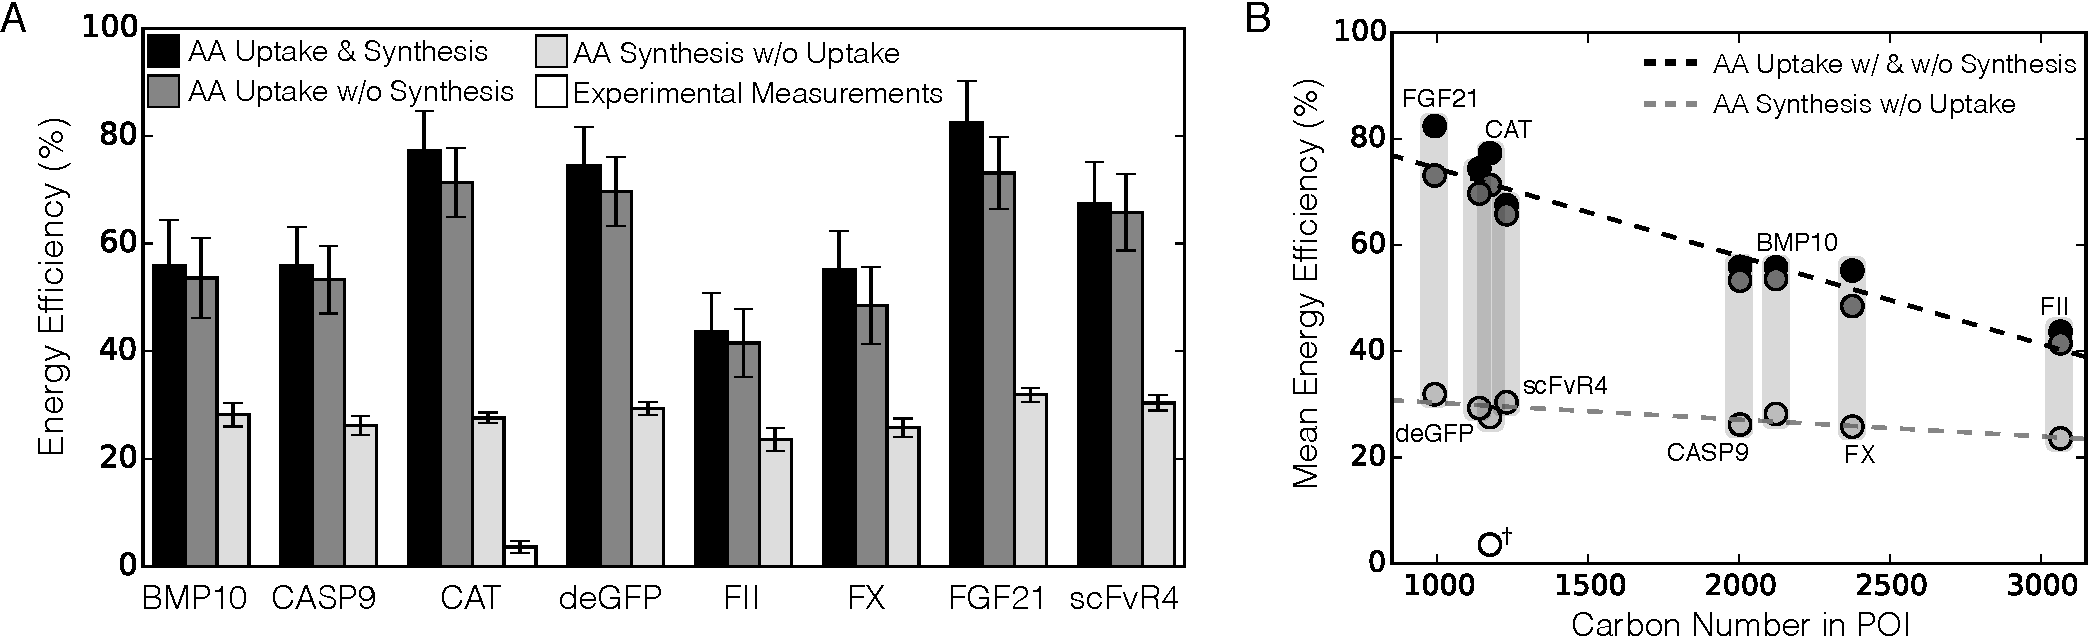
\includegraphics[width=1.00\textwidth]{./Figures/Energy.pdf}
\caption{CFPS energy efficiency of eight proteins for four cases. Amino acid uptake and synthesis (black), AA uptake without synthesis (dark grey), AA synthesis without uptake (light grey), and constrained by experimental measurements, for CAT only (white). A. Energy efficiency (Error bars represent the 95\% CI of the ensemble). B. Mean energy efficiency versus the carbon number for each corresponding protein. Trendline of energy efficiency versus carbon number (black dotted line) for first two cases (y = -1.65$\cdot$10\textsuperscript{-2}x+90.95; R\textsuperscript{2} = 0.91) and trendline for AA synthesis without uptake (grey dotted line; y = -3.18$\cdot$10\textsuperscript{-3}x+33.48; R\textsuperscript{2} = 0.78). Dagger: constrained by experimental measurements and excluded from trendline.}
\label{fig:Energy}
\end{figure}


\subsubsection{Yield}
The mean carbon yield was inversely proportional to protein size and varied between 40-57\% for the proteins sampled (Fig.~\ref{fig:Yield}).
The same inverse qualitative trend was observed as for energy efficiency.
%The cases supplemented with amino acids in the media showed the highest carbon yield.
There was a drop in carbon yield by about 7\% once amino acids were not available; this is most likely because glucose was utilized to synthesize the necessary amino acids for each protein as well as power the system.
%To determine the carbon contribution from each substrate (glucose and amino acids) we examined the carbon flux going toward the production of deGFP for all three cases (Table \ref{tbl:yield_breakdown}).
For the first case, the system relied on a mixture of glucose and some amino acids for each protein with a carbon yield of 58.2 $\pm$ 2.3\% for CAT.
Once amino acid synthesis reactions were blocked in the network (second case), the carbon yield dropped to 57.1 $\pm$ 2.2\% for CAT.
Only the necessary amount of amino acids was used for the production of the protein of interest; thus, it may be hypothesized that all the glucose was used to power CFPS and did not contribute to the carbon yield.
In that case, the carbon yield without glucose contribution would be 100\%.
%Finally, for the third case (without amino acids supplemented), the carbon yield was reduced to 51.1 $\pm$ 1.8\% for CAT, and the system used about twice the amount of glucose as in the first two cases.
%In this case, glucose was used to synthesize amino acids and provide the energy necessary to power transcription and translation; this trend was seen across all proteins.
In the experimentally constrained case, CAT was produced with a carbon yield of 6.2\% compared to the theoretical maximum of 58.2\%.
This decrease in carbon yield suggests inefficiencies in CFPS that can potentially be improved.
ssFBA assumes a psuedo steady state; thus, intermediate metabolites cannot accumulate within the cell-free extract.
In addition, ssFBA is solved by maximizing the flux through the protein production reaction.
Therefore, carbon flux will travel through the network to optimize the maximum flux through the protein synthesis reaction.
In examining the experimental dataset, there is a high accumulation of organic acids, especially acetate, pyruvate and lactate.
The experimental performance could be improved by diverting this carbon toward the protein of interest by knockouts during the cell-free extract preparation.
\begin{figure}[t!]
\centering
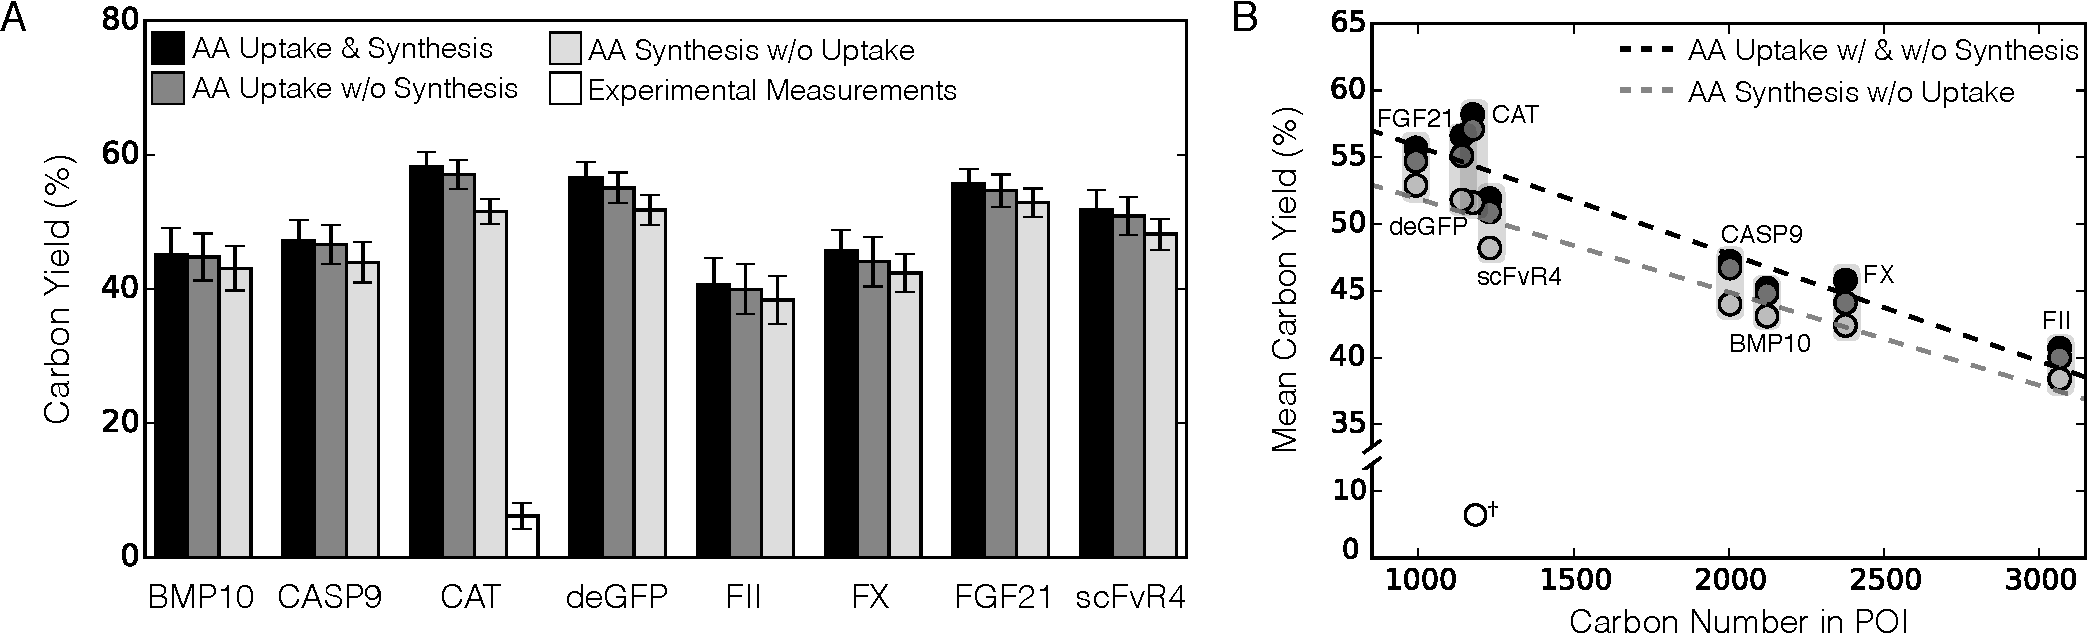
\includegraphics[width=1.00\textwidth]{./Figures/Yield.pdf}
\caption{CFPS carbon yield of eight proteins for four cases. Amino acid uptake and synthesis (black), AA uptake without synthesis (dark grey), AA synthesis without uptake (light grey), and constrained by experimental measurements, for CAT only (white). A. Energy efficiency across the ensemble (error bars represent the 95\% CI). B. Mean energy efficiency versus the carbon number for each corresponding protein. Trendline of energy efficiency versus carbon number (black dotted line) for first two cases (y = -8.03$\cdot$10\textsuperscript{-3}x+63.83; R\textsuperscript{2} = 0.95) and trendline for AA synthesis without uptake (grey dotted line; y = -6.98$\cdot$10\textsuperscript{-3}x+58.86; R\textsuperscript{2} = 0.90). Dagger: constrained by experimental measurements and excluded from trendline.}
\label{fig:Yield}
\end{figure}
%Next we investigated the effect of the carbon number of each protein on the carbon yield (Fig.~\ref{fig:Yield}B).
%The proteins with the lowest carbon number had the highest yield and the higher carbon number proteins had a lower carbon yield within each case.
A single trendline was formulated for the cases where amino acids were supplied in the media since they had similar performance, while another trendline was formulated for when amino acids were not available (Fig.~\ref{fig:Yield}B).
The trendlines showed good predictability for estimating carbon yield for a certain range of potein size (R\textsuperscript{2} = 0.95 with amino acids and R\textsuperscript{2} = 0.90 without amino acids), regardless of the type of promoters used.
However, as the protein size increased, the carbon yield decreased, suggesting that larger proteins may be less feasible for cell-free production.
Thus, we examined the parameters that had the most significant effect on cell-free productivity, energy efficiency, and carbon yield in order to optimize CFPS performance.

\subsection{Sensitivity analysis}
The translation rate had the highest effect on protein productivity, whereas oxygen followed by substrate uptake had the highest effect on energy efficiency and carbon yield (Fig.~\ref{fig:SI}).
To better understand the effect of substrate utilization and the transcription/translation parameters on CFPS performance we performed global sensitivity analysis on the productivity and energy efficiency for CAT, a representative protein (Fig.~\ref{fig:SI}), as well as on the carbon yield which followed the same trend of significance as energy efficiency (available in Supporting Information).
In examining productivity performance (Fig.~\ref{fig:SI}A), the significance of transcription/translation parameters was fairly constant across all three cases, with the rate of translation being the most significant.
As expected, this showed that the translation rate was instrumental for productivity, and should be the first step investigated during optimization, prior to examining transcription parameters.
Underwood and coworkers have also shown that an increase in ribosome levels did not significantly increase protein yields or rates; however, adding elongation factors increased yields by 23\% at 30 minutes \cite{2005_underwood_biotech}.
In addition, Li et al. have increased productivity of firefly luciferase by 5-fold in CFPS systems by adjusting factors that affect transcription and translation such as elongation factors, ribosome recycling factor, release factors, chaperones, BSA, and tRNAs \cite{2014_li_PlosOne}.
In examining substrate utilization, glucose uptake was not seen to be very important for productivity in the cases with amino acid supplementation, but its significance increased when amino acids were not available.
This makes sense, as amino acid synthesis from glucose became the only way to power protein synthesis.
On the other hand, amino acid uptake only showed significance for the case where amino acids synthesis reactions were blocked, as it was the only source of amino acids for CAT synthesis.
\begin{figure}[t!]
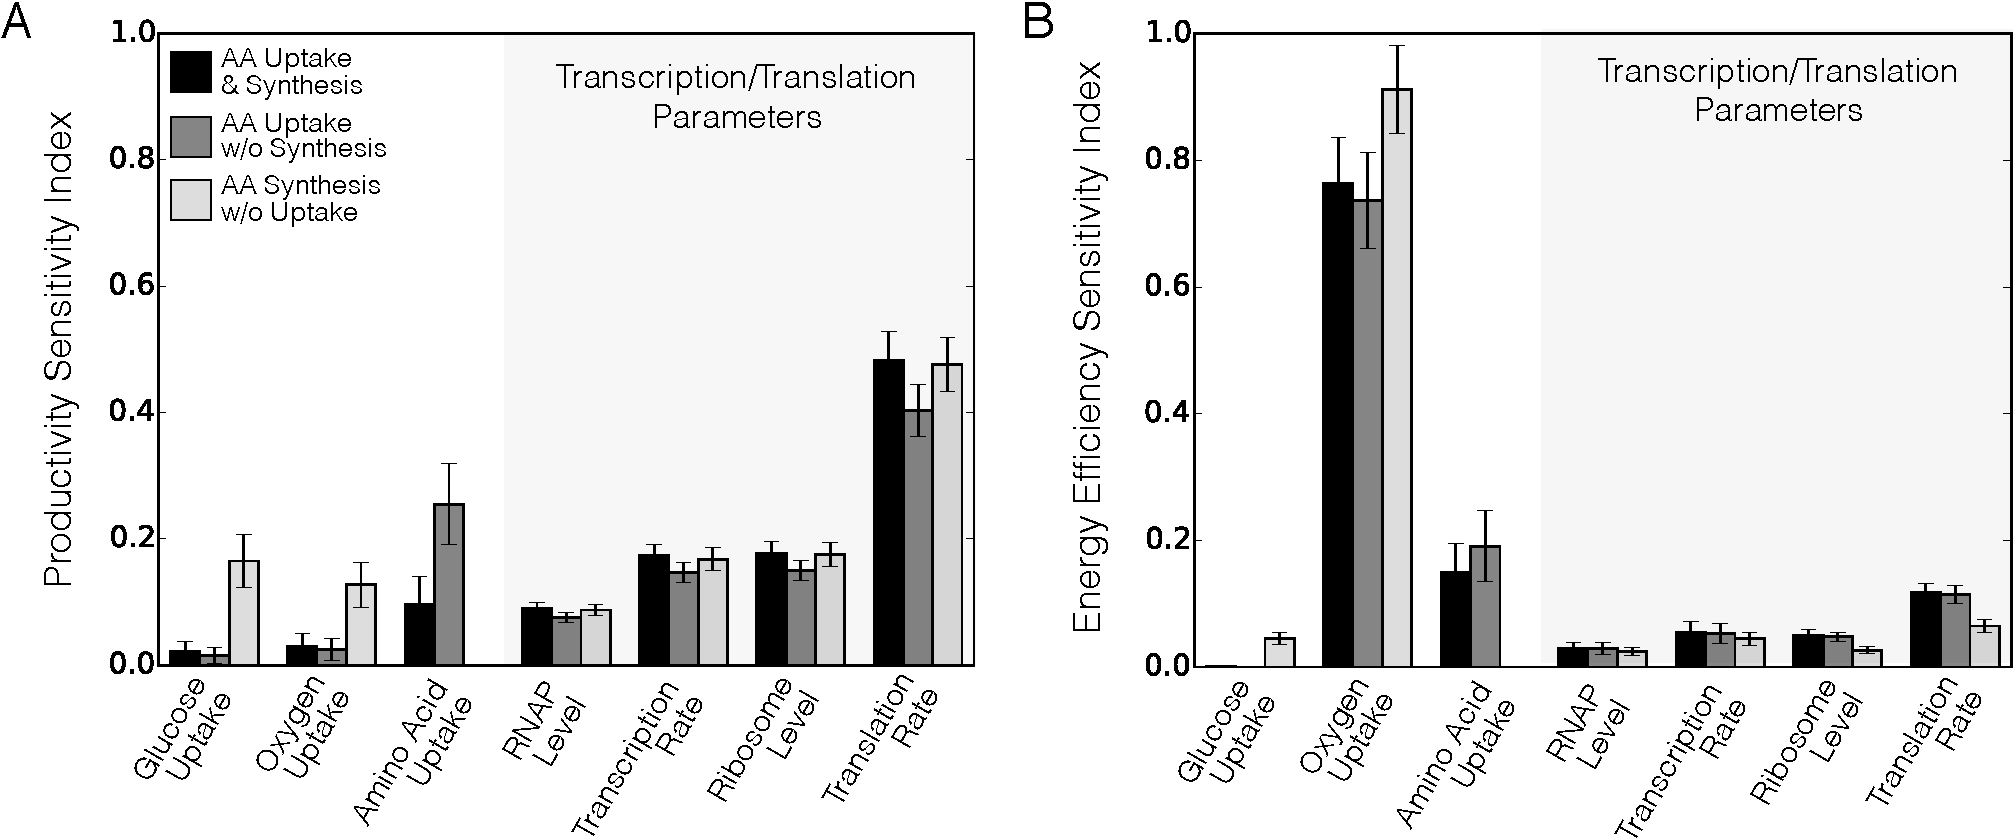
\includegraphics[width=1.00\textwidth]{./Figures/Sensitivity.pdf}
\caption{Total order sensitivity of deGFP productivity (A) and energy efficiency (B) to specific uptake rates and transcription/translation parameters for three cases: amino acid uptake and synthesis (black), amino acid uptake without synthesis (dark grey), and amino acid synthesis without uptake (light gray). Error bars represent a 95\% CI on the sensitivity index.}
\label{fig:SI}
\end{figure}

When considering energy efficiency performance (Fig.~\ref{fig:SI}B), the oxygen uptake rates were the most important for all cases while the sensitivity of the transcription/translation parameters decreased.
The transcription/translation parameters had the same trend as for productivity, where the translation rate was the most sensitive compared to the other transcription/translation parameters and showed significance across all cases.
Oxygen uptake was the most significant for energy efficiency, since it was responsible for oxidative phosphorylation, the most efficient pathway for energy generation.
Across all cases, substrate utilization (amino acid uptake and glucose) was shown to be the next most important as these substrates contributed to the energy efficiency of CAT synthesis.
In cases where amino acids were supplied, amino acid uptake was significant, as without it, energy was required to synthesize amino acids for the protein of interest.
Glucose uptake was only important when amino acids were not available, since it was the only source of carbon for protein synthesis and energy generation.
%This resulted in a tradeoff between energy generation to power transcription/translation and amino acid synthesis required to assemble the protein of interest.
Jewett and coworkers have reported that oxidative phosphorylation still operated in cell-free systems, and that yield decreased from 1.5-fold to 4-fold when oxidative phosphorylation reactions were knocked out in pyruvate-powered CFPS \cite{Jewett:2008aa}.
It is unknown how active oxidative phosphorylation is compared to in \textit{in~vivo} systems.
To investigate this further we compared CAT carbon yield to oxidative phosphorylation flux (Fig.~\ref{fig:oxphos_yield}).
Interestingly, oxidative phosphorylation had a strong effect on the carbon yield in all cases.
The cases where amino acids were supplied followed the same trend: ranging from a carbon yield of 20\% to 58\%, depending on the oxidative phosphorylation activity.
Once amino acids were removed from the media, the carbon yield dropped to about 10\%, and reached a maximum of 52\%.
When amino acids are not avialable in the media, a lower carbon yield was expected for the same oxidative phosphorylation flux, since carbon must be utilized for energy generation and amino acid biosynthesis.
In all cases, whenever the carbon yield was below its theoretical maximum, there was an accumulation of acetate and lactate, resulting in the lower carbon yield.
The experimental dataset exhibits a mixture of acetate and lactate accumulation during CAT synthesis, which shows that CFPS is not operating in a fully aerobic state.
Glucose can not be fully oxidized and therefore fermentation pathways are used. 
Oxidative phosphorylation relies on electron transport from membrane vesicles, however CFPS has no cell membrane, thus it is expected CFPS has limited oxidative phosphorylation activity.
The addition of phosphate showed an increase in CAT yield; however, it is unclear whether the addition of phosphate enhances oxidative phosphorylation, inhibits phosphatase reactions, or both \cite{Jewett:2008aa}.
Interestingly, the addition of NADH did not increase the rate of protein synthesis, since the concentration of ATP was most likely saturated.
An alternative strategy may be the inhibition of anaerobic processes in cell-free, in order to minimize unwanted byproducts such as acetate and lactate.
%Thus, it is interesting to see how much of the energetic needs of the system are met by oxidative phosphorylation and how much from anaerobic processes.
\begin{figure}[t!]
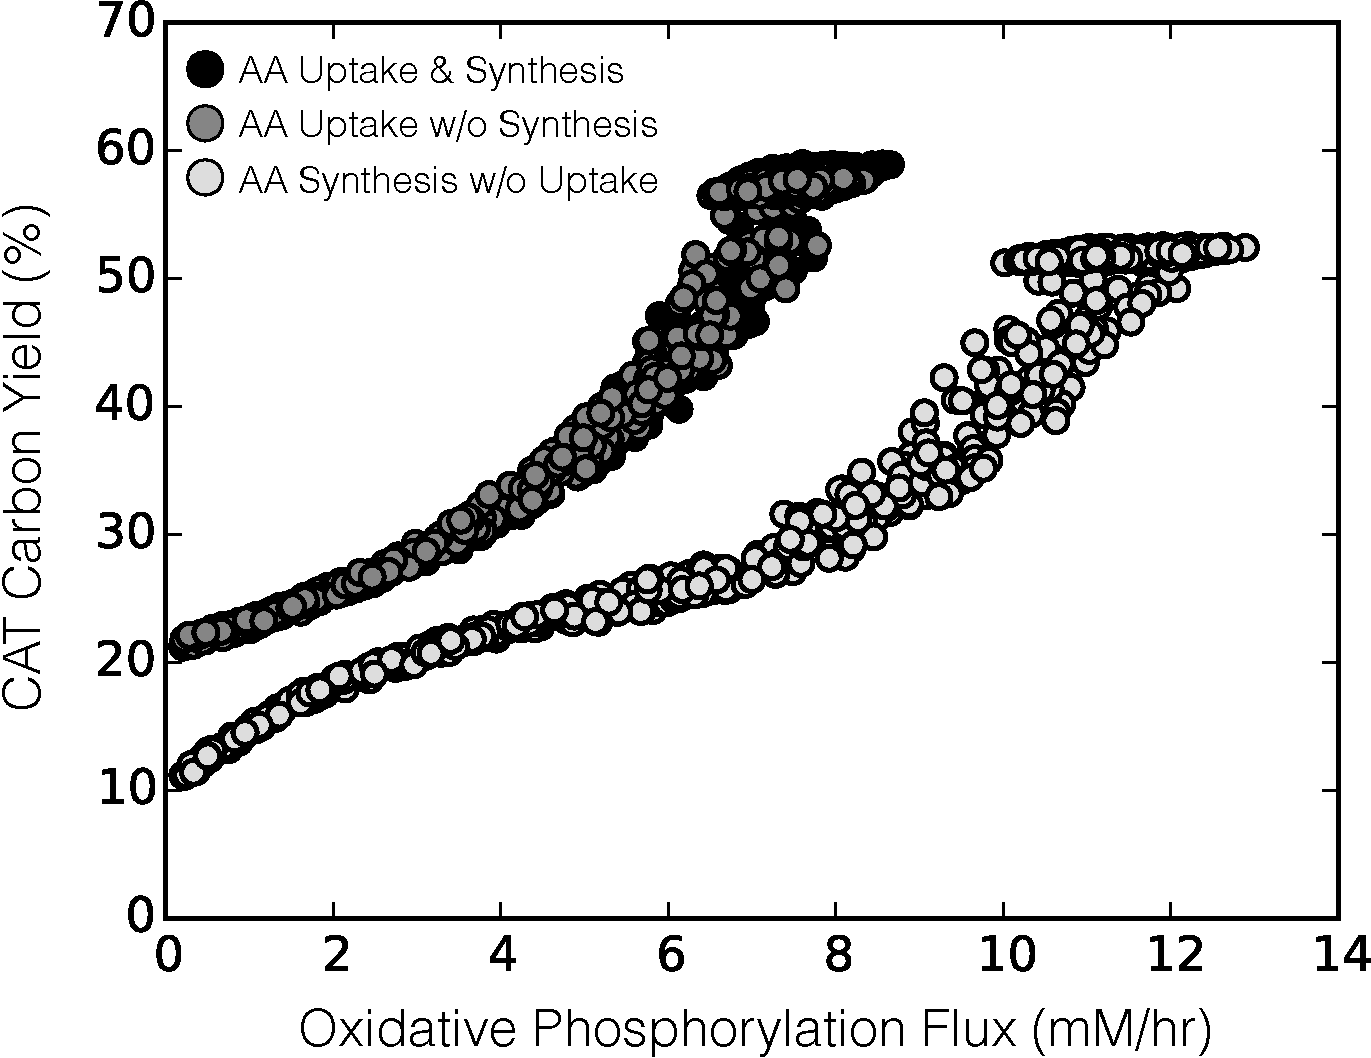
\includegraphics[width=0.7\textwidth]{./Figures/Ox_yield.pdf}
\caption{deGFP carbon yield versus oxidative phosphorylation flux, across an ensemble of 1000 ssFBA solutions, for three cases: amino acid uptake and synthesis (black), amino acid uptake without synthesis (dark grey), and amino acid synthesis without uptake (light gray).}
\label{fig:oxphos_yield}
\end{figure}

\subsection{Flux distribution}
To investigate the differences between the three cases, we compared the flux distributions for CAT production predicted by ssFBA simulations (Fig.~\ref{fig:flux}).
\begin{figure}[t!]
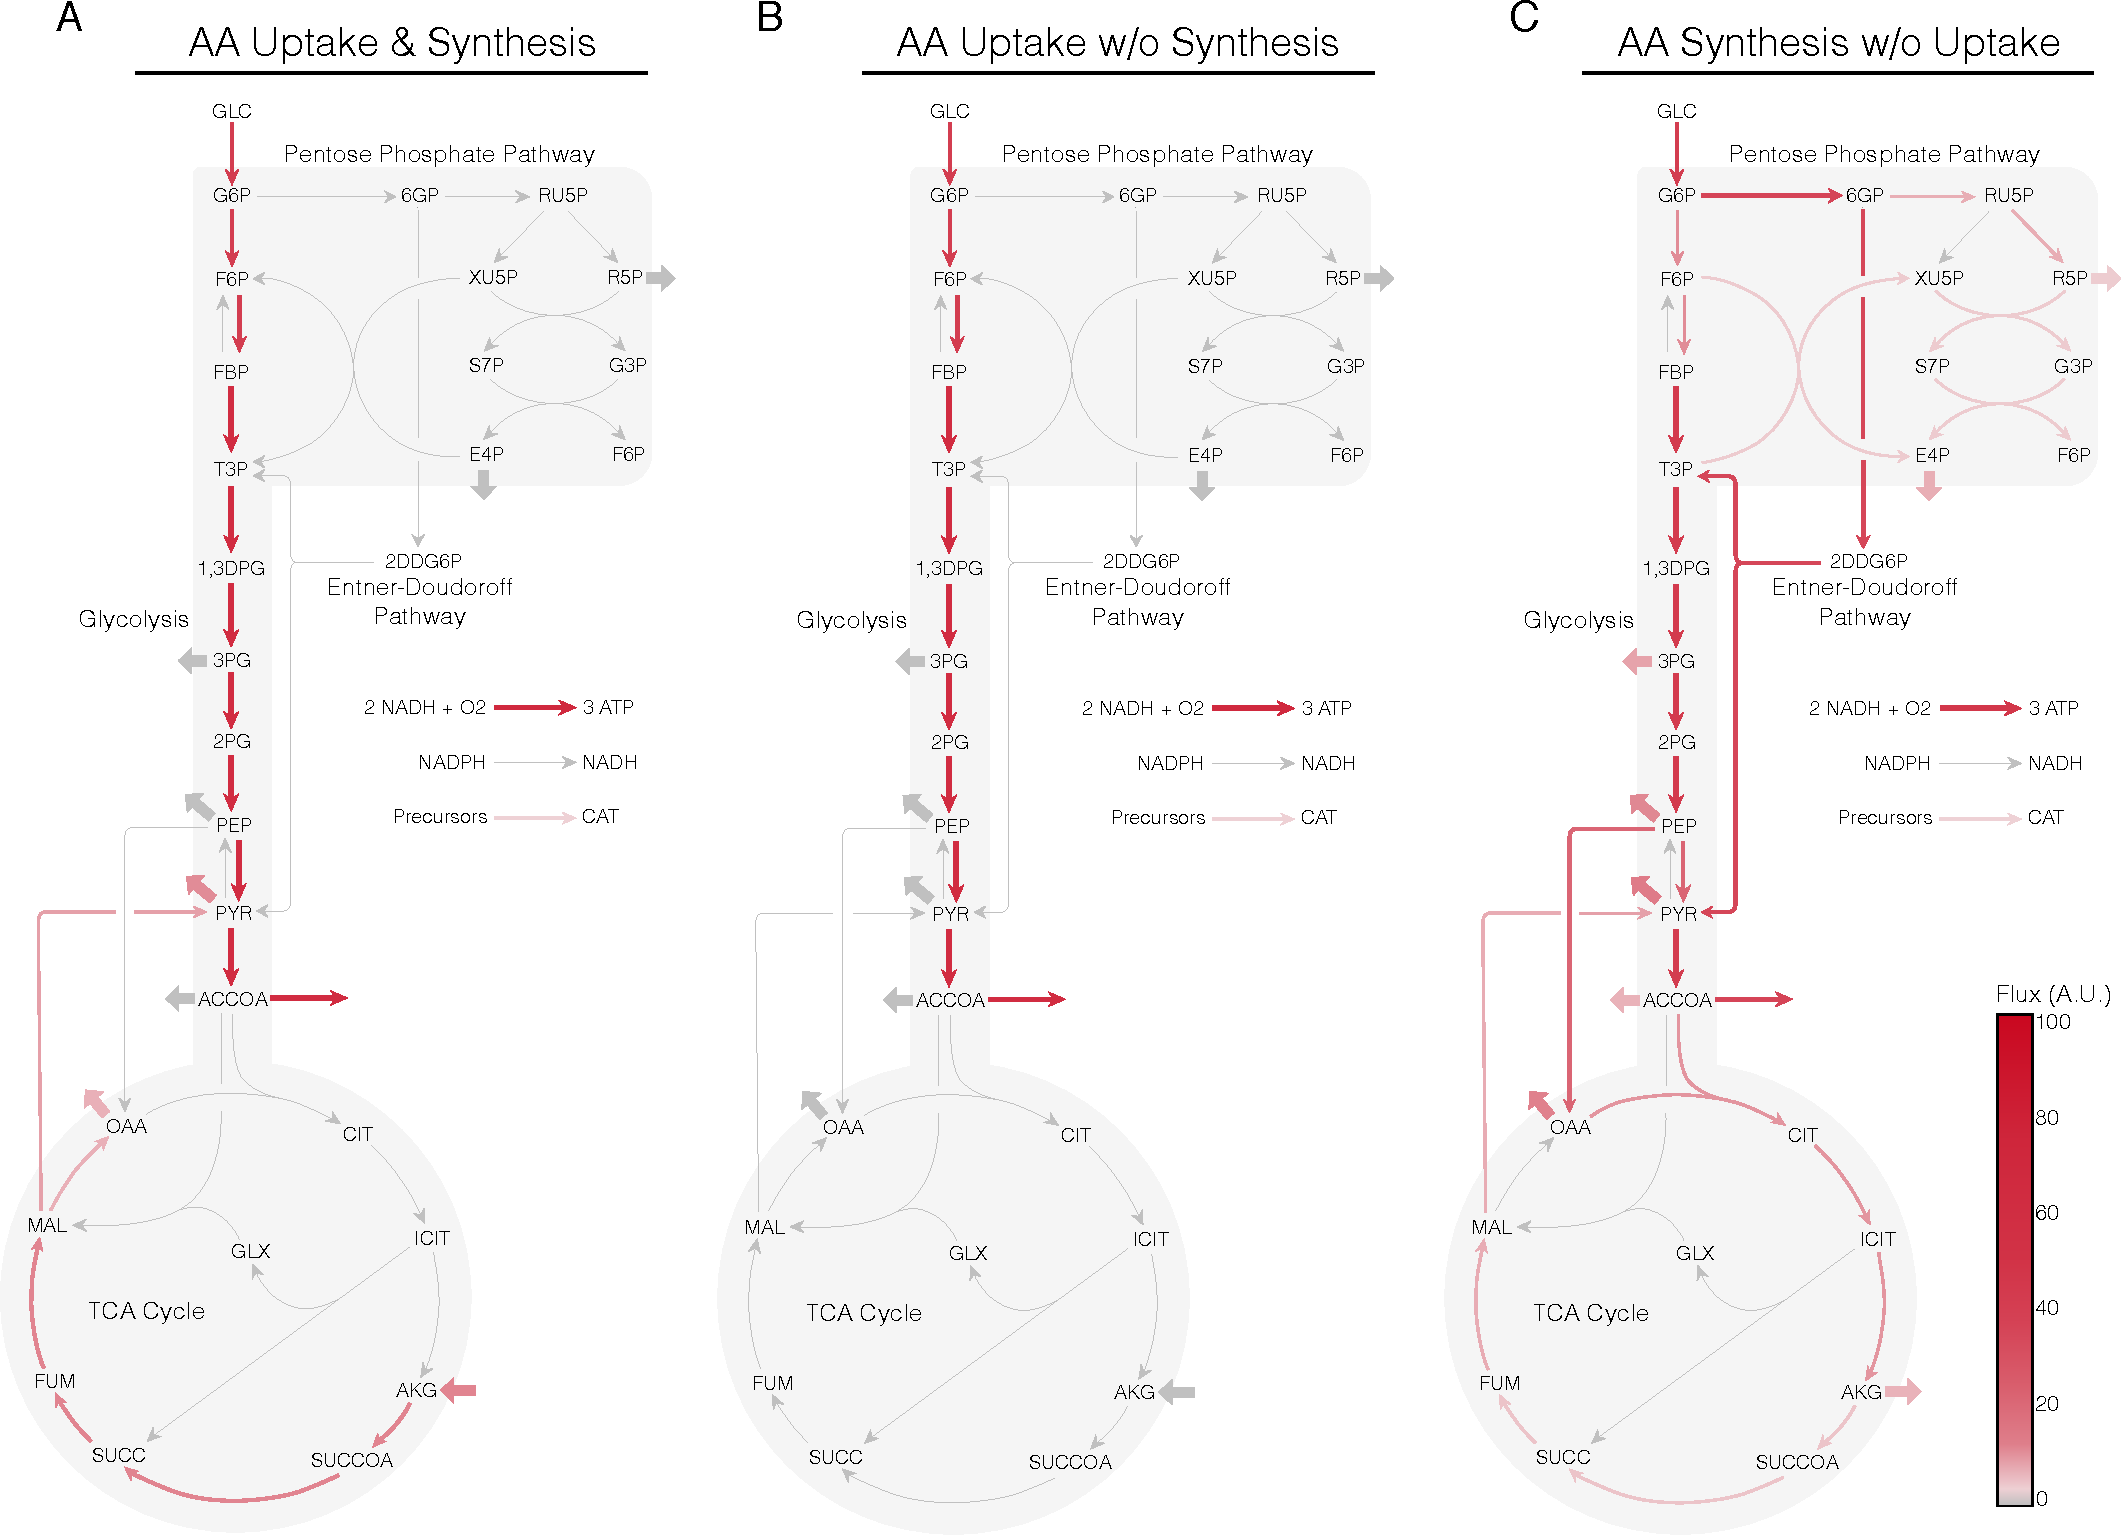
\includegraphics[width=1.00\textwidth]{./Figures/Flux.pdf}
\caption{Flux profile for glycolysis, pentose phosphate pathway, Entner-Doudoroff pathway, TCA cycle, and oxidative phosphorylation, for three different cases: (A) amino acid uptake and synthesis, (B) amino acid uptake without synthesis, and (C) amino acid synthesis without uptake. Mean flux across the ensemble, normalized to glucose uptake flux. Thick arrows indicate flux to or from amino acids.}
\label{fig:flux}
\end{figure}
In the cases supplied with amino acids (Fig.~\ref{fig:flux}A-B), glucose traveled to acetyl-coenzyme A that generated NADH for oxidative phosphorylation to energize CFPS.
Interestingly, in the first case with amino acid synthesis reactions, ssFBA relied on a combination of glucose and amino acids to power the system
Amino acids rather than glucose powered the TCA cycle via glutamate to alpha-ketoglutarate which traveled to oxaloacetic acid and pyruvate for additional amino acid biosynthesis.
In the case where amino acid synthesis reactions were blocked (Fig.~\ref{fig:flux}B), ubiquinone was generated via \textit{nuo} to power oxidative phosphorylation, instead of relying on the TCA cycle.
Once the energy requirements for transcription and translation were met, amino acids were taken from the media to assemble the protein of interest.
These first two cases where amino acids were available had similar performance with a correlation of 0.99 between their flux distributions and were comparable in terms of productivity, energy efficiency and carbon yield for all proteins.
%This is most likely due to the efficient utilization of carbon to energize CFPS without the burden of amino acid biosynthesis.
In the case where amino acids must be synthesized, there was a drop in the performance metrics of energy efficiency and carbon yield compared to the cases where amino acids are avialble.
The flux distribution had a correlation of 0.90 when compared to both cases where amino acids were avaialbe. 
This drop in performance is due to the burden of synthesizing amino acids, which require NADPH.
This leads to the relatively high flux in the first step of the pentose phosphate pathway to generate NADPH, thus, less NADH is available for oxidative phosphorylation.
The performance metrics and sensitivity analysis suggest that efficient energy generation via oxygen uptake is essential to higher energy efficiency and carbon yields.
%Thus, removing anaerobic enzymes during the cell-free extract preparation could potentially improve CFPS performance and protein yield.

The case constrained by experimental measurements (Fig. \ref{fig:flux_exp}), had the highest correlation of 0.66 with the flux distribution from the case supplied with no amino acids and a correlation of 0.52 with the cases supplied with amino acids.
Thus there are some differences in the flux distribution compared to the optimum solutions which may provide some insight to improve CFPS performance. 
Metabolic fluxes were constrained by experimental measurements (available in Supporting Information) where available for the first hour which constrained the solution space of ssFBA to have a more realistic depiction of the flux distribution.
The central carbon organic acids showed good agreement with the data (Fig.~\ref{fig:flux_exp}B).
Only certain amino acid synthesis reactions were blocked since during the growth of \emph{E.~coli} not all amino acids were supplied (see Materials and Methods).
During the cell-free reaction all amino acids were supplied, however glucose still traveled through all the major pathways, and the same metabolic precursors were still utilized for amino acid biosynthesis.
In this case, it is unclear which substrate (glucose or amino acids) is used to power CFPS and may in fact be a combination of both.
The optimum solutions only produced the required amount of amino acids necessary, however in examining the measurements there is an accumulation of alanine and glutamine which may explain some of the differences in the correlations of the flux distributions.
Accumulation of pyruvate, lactate, acetate, and other organic acids can be seen (Fig.~\ref{fig:flux_exp}B) and shows an inefficiency of carbon utilization.
\begin{figure}[t!]
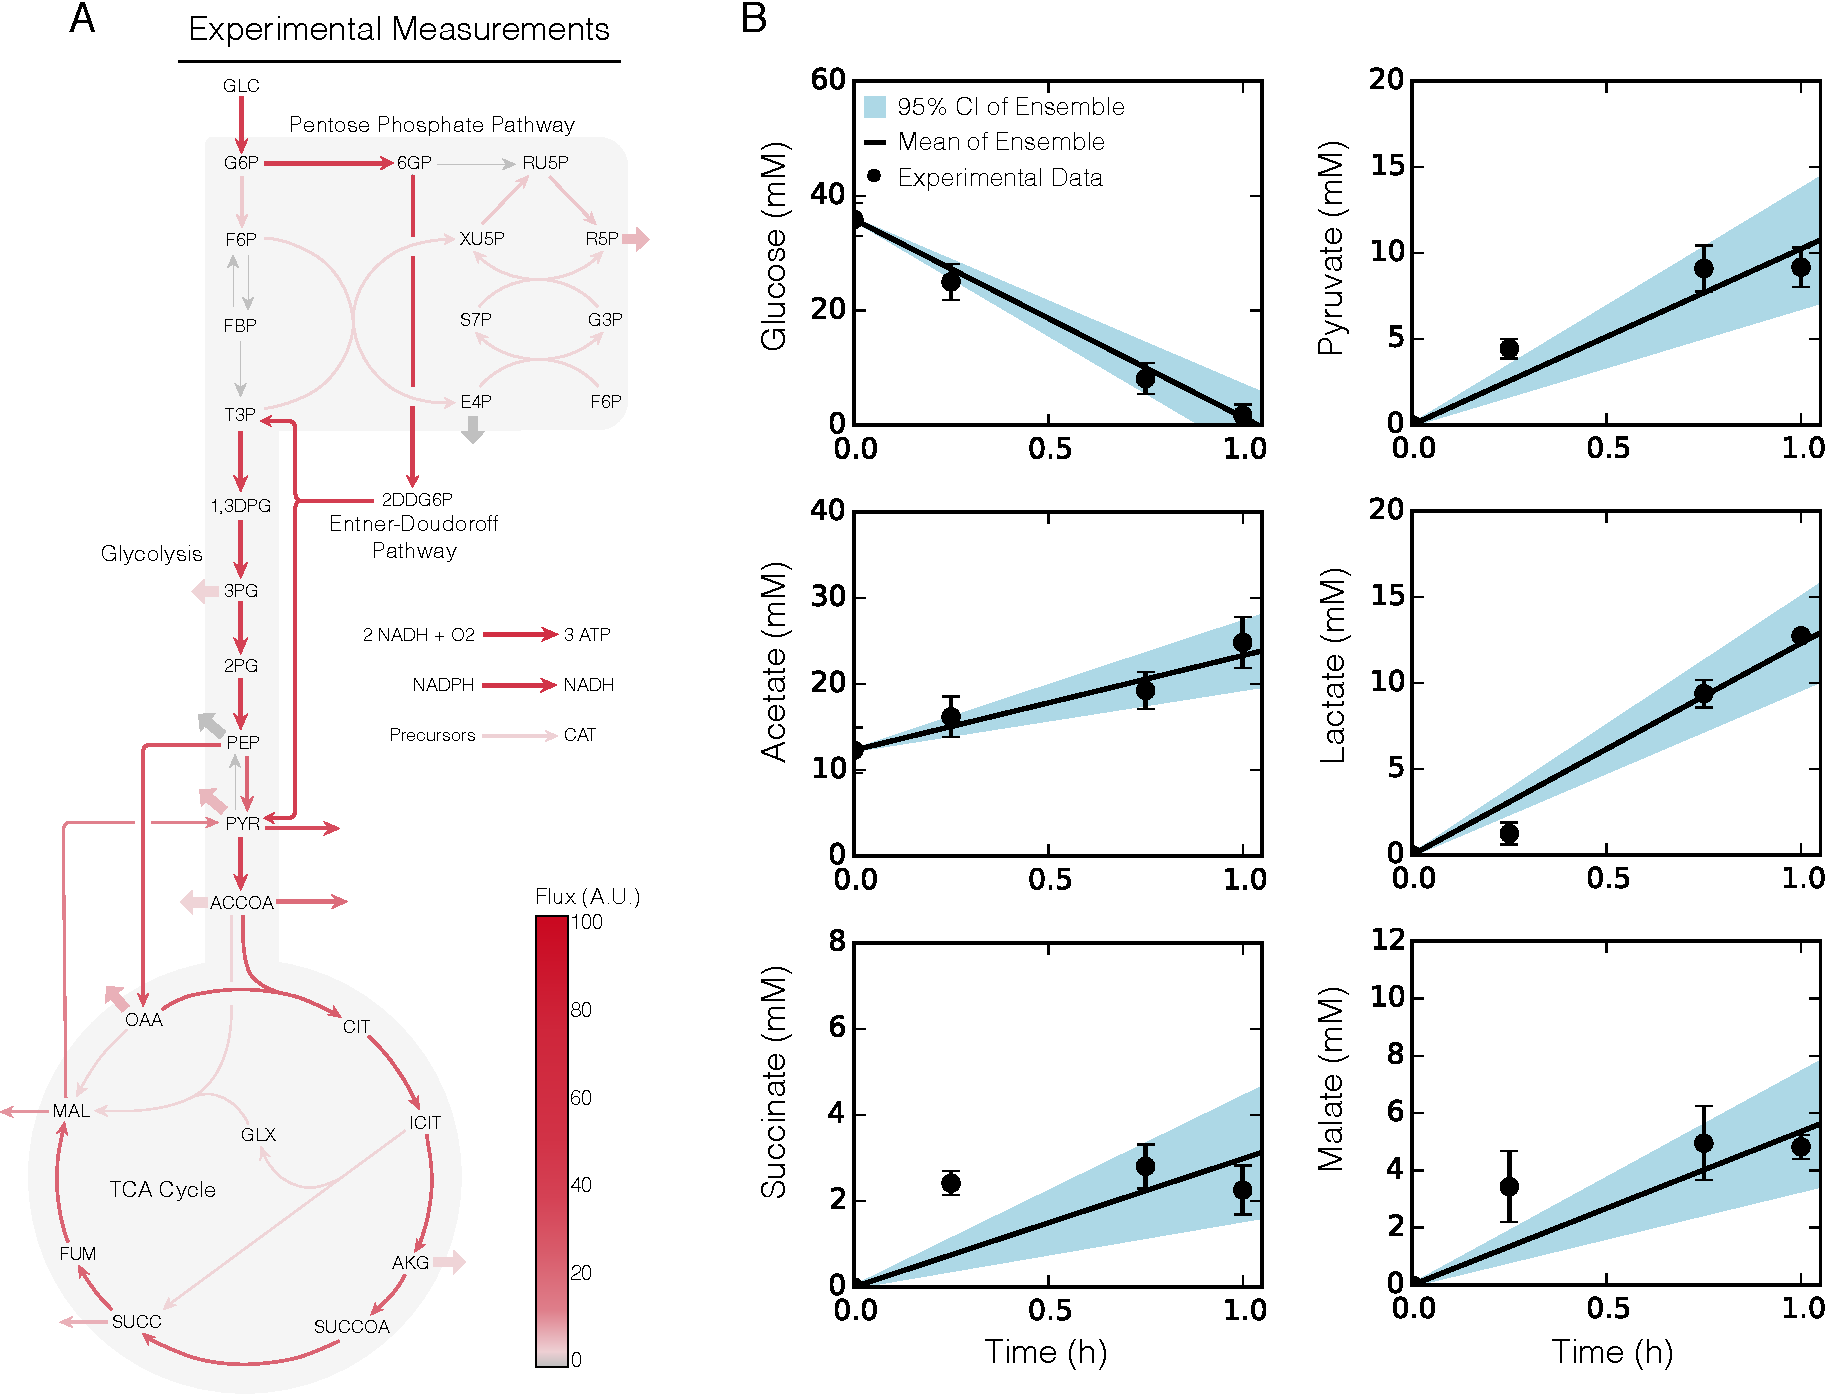
\includegraphics[width=1.00\textwidth]{./Figures/Exp_flux.pdf}
\caption{ssFBA simulation of CAT production for an experimentally constrained case. (A) Flux profile for glycolysis, pentose phosphate pathway, Entner-Doudoroff pathway, TCA cycle, and oxidative phosphorylation.  Mean flux across the ensemble, normalized to glucose uptake flux. Thick arrows indicate flux to or from amino acids. (B) Central carbon metabolite measurements versus ssFBA simulations over a one hour time course.}
\label{fig:flux_exp}
\end{figure}

Despite the constraints by experimental measurements, it is difficult to calculate the physiological flux distribution of metabolism (Fig.~\ref{fig:norm}) 
For example, there is a high flux through the Entner-Douodoroff pathway, but this is likely non-physiological, and simply an artifact of the optimal solution of ssFBA.
A knockout of the Entner-Doudoroff pathway has no effect on the norm productivity of CAT compared to no knockouts (Fig.~\ref{fig:norm}A).
In addition, pairwise knockouts of Entner-Doudoroff and most subgroups in the network result in the same optimal solution of CAT productivity.
However, there is a difference in the flux distribution with these knockouts (Fig.~\ref{fig:norm}B), ssFBA will reroute the flux to optimize the objective function.
Interestingly, a single group knockout of glycolysis/gluconoeogenesis, glutamate/glutamine biosynthesis, alanine/aspartate/asparagine biosynthesis was detrimental to CAT productivity.
Flux balance analysis has been shown to have multiple alternative optimal solutions with flux variablitiy analysis and mixed-integer linear programming resulting in a poor depiction of the physiological flux distribution \cite{LEE2000711, Mahadevan2003264, Schuetz119}. 
In our case, ssFBA reached the same optimal solution of CAT productivity for 73\% of the pairwise group knockouts. 
To determine which reactions occur in CFPS, adding thermodynamic feasibility constraints to reactions may result in a better depiction of the flux distribution \cite{Henry:2007,Hamilton:2013}.
It would also be interesting to track the carbon flux using C\textsuperscript{13} labeling in CFPS and constrain branch reactions in ssFBA to the resulting measurements, a method that has been shown to represent the flux distribution for \emph{in~vivo} processes well \cite{Zamboni:2009}.
\begin{figure}[t!]
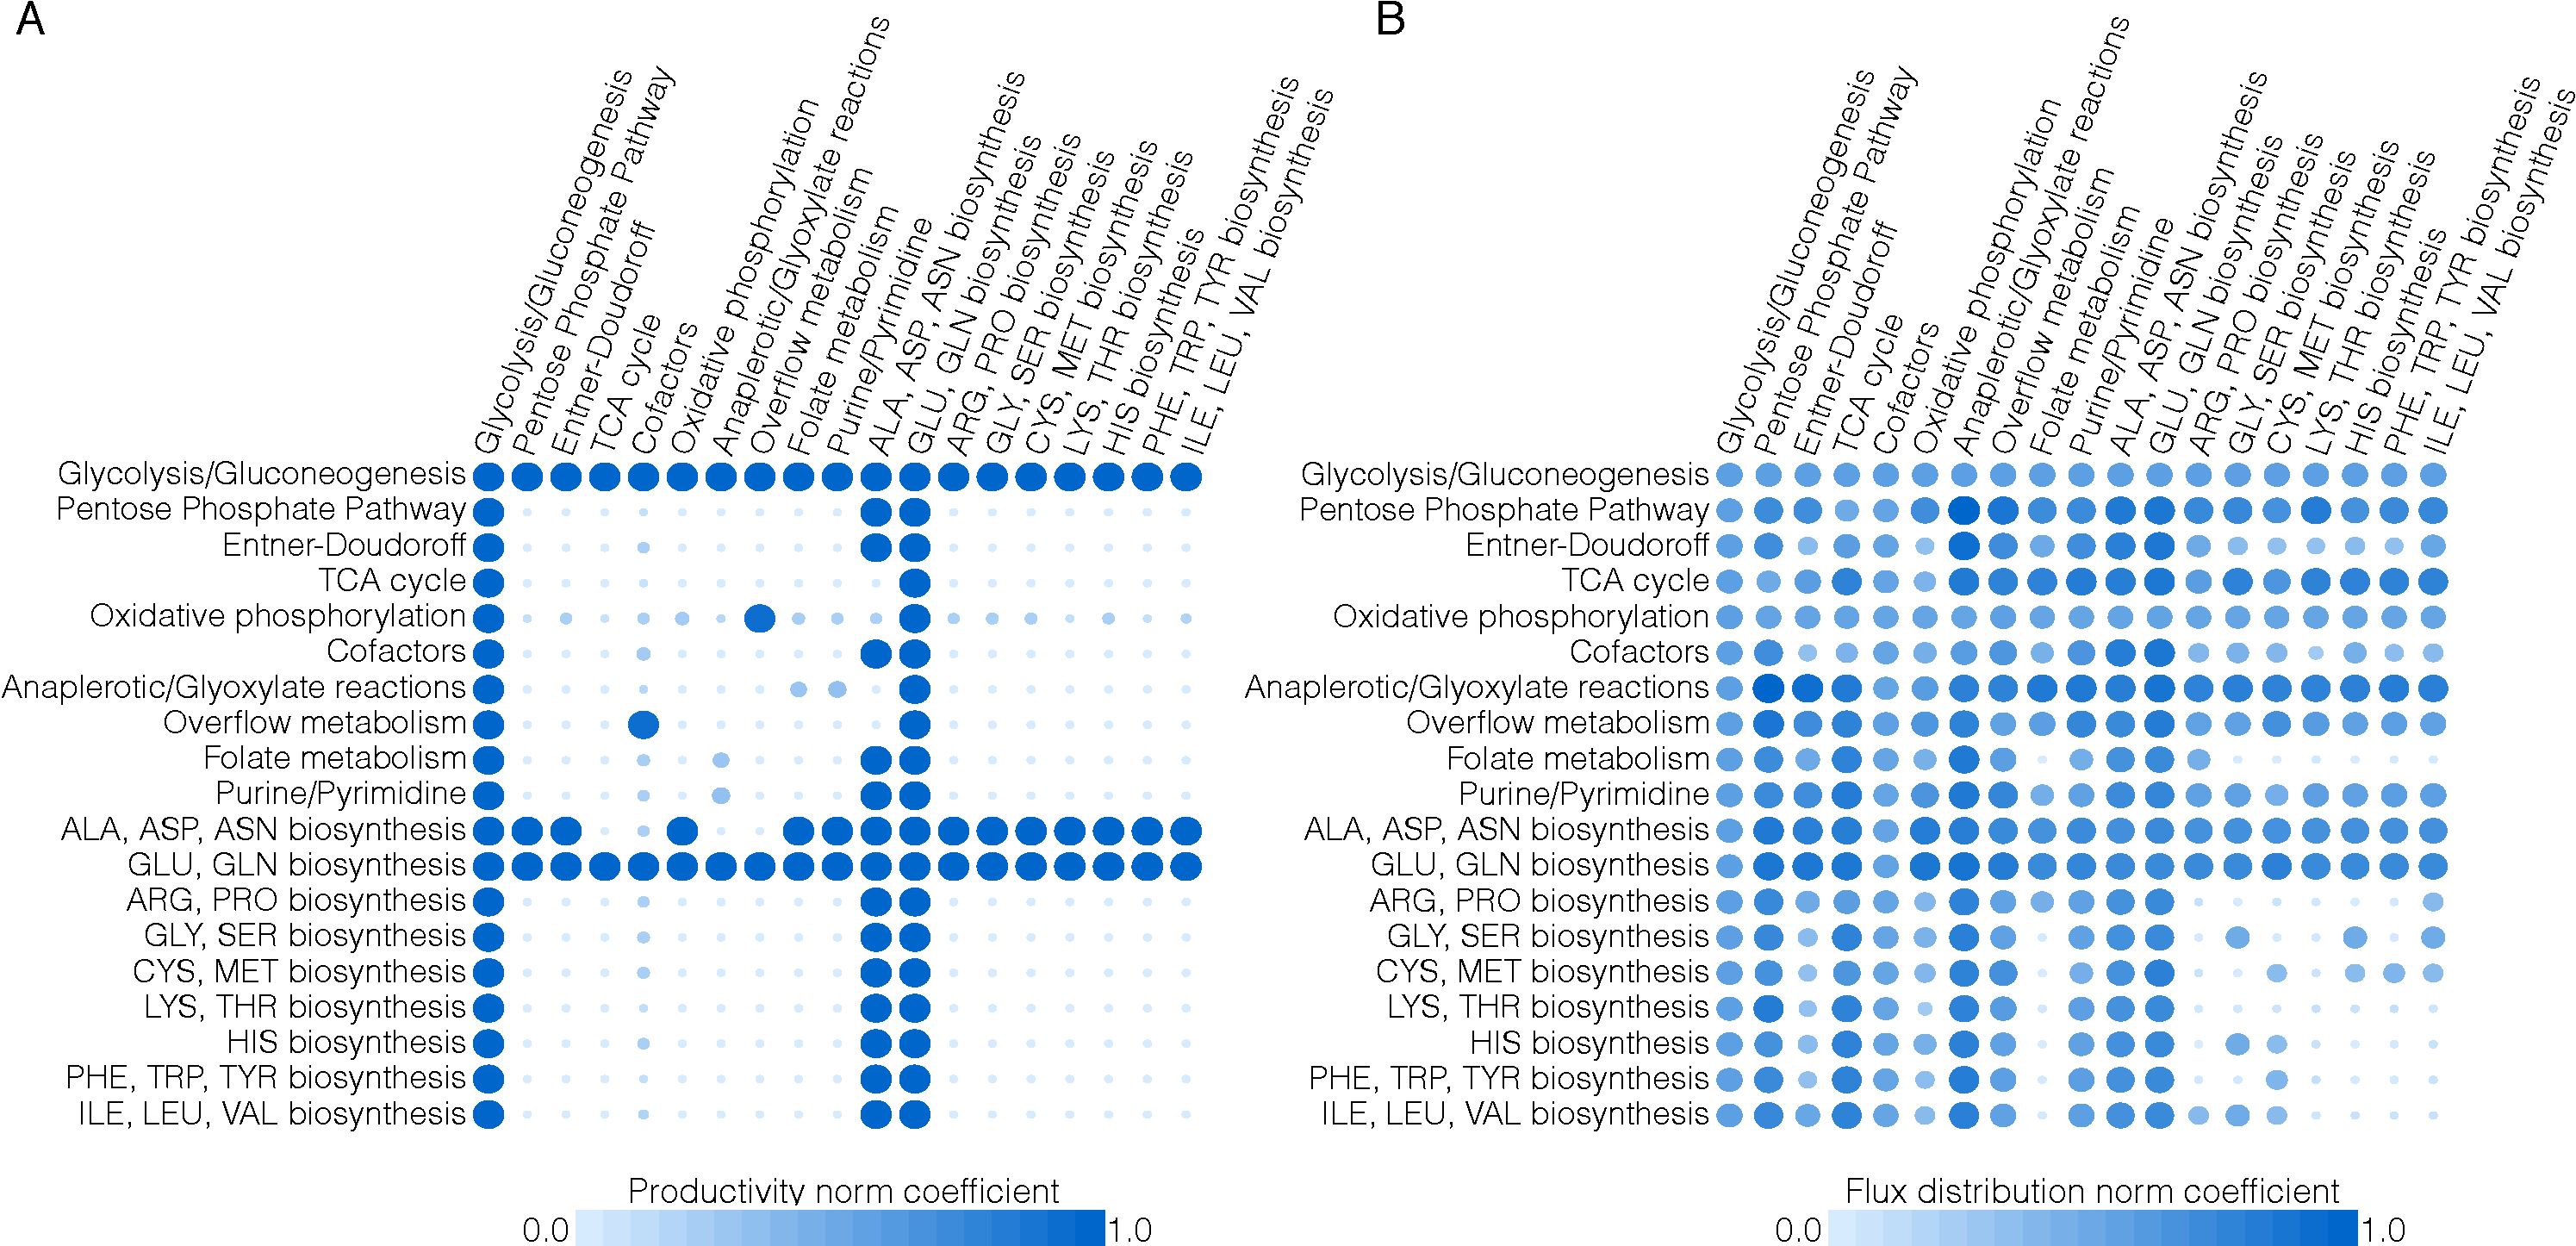
\includegraphics[width=1.0\textwidth]{./Figures/Norm.pdf}
\caption{The norm effect of pairwise knockouts of subgroups in the cell-free network (A) CAT productivity norm compared to no knockouts in the experimentally constrained case. (B) Flux distribution norm compared to no knockouts in the experimentally constrained case.}
\label{fig:norm}
\end{figure}

Taken together, we developed a sequence specific constraints based modeling approach to evaluate the performance of synthetic circuits in an \emph{E.~coli} CFPS system for a range of different proteins and three different cases.
We have shown first principle predictions for protein production of deGFP and CAT in agreement with experimental measurements, under two different promoters and two different cell-free extract systems, with few adjustable parameters in the promoter models taken from literature.
This modeling approach suggested trends for productivity, energy efficiency and carbon yield as a function of carbon number.
Furthermore, global sensitivity analysis identified oxygen uptake as being instrumental for maintaining a high energy efficiency and carbon yield.
The translation rate was identified as the rate limiting step for productivity.
The model also suggested that cell-free systems can simultaneously operate aerobically and anaerobically, which can lead to inefficient production and should be addressed to optimize energy efficiency and carbon yield.
In conclusion, sequence specific constraints based modeling offers a novel means to \emph{a~priori} estimate the performance of cell-free synthetic circuits.

\clearpage

\section*{Materials and Methods}

\subsection*{Glucose/NMP cell-free protein synthesis.}
The glucose/NMP cell-free protein synthesis reactions were performed at a volume of 15 $\mu$L in 1.5-mL eppendorf tubes and incubated in a humidified incubator.
Plasmid pK7CAT was used as the DNA template for chloramphenical acetyl transferase (CAT) expression by placing the \emph{cat} gene between the T7 promoter and the T7 terminator \cite{Kigawa1995}.
The plasmid was isolated and purified using a Plasmid Maxi Kit (Qiagen, Valencia CA).
Cell-free protein synthesis of CAT protein was performed at 37 $^{\circ}$C for 3 h.

S30 extract was prepared from E. coli strain KC6 (A19 $\Delta$tonA $\Delta$tnaA $\Delta$speA $\Delta$endA $\Delta$sdaA $\Delta$sdaB $\Delta$gshA met+).
This K12-derivative has several gene deletions to stabilize amino acid concentrations during the cell-free reaction.
The KC6 strain was grown to approximately 3 OD595 in a 10-L fermenter (B. Braun, Allentown PA) on defined media with glucose as the carbon source and with the addition of 13 amino acids (alanine, arginine, cysteine, serine, aspartate, glutamate, and glutamine were excluded) \cite{Zawada:2003}.
Crude S30 extract was made as previously described \cite{Jewett:2002}.

The standard protein synthesis reaction was conducted according to the PANOxSP protocol with slight modifications from that described previously \cite{BIT:BIT20026}.
Unless otherwise noted, all reagents were purchased from Sigma (St. Louis, MO).
The initial mixture includes 1.2 mM ATP; 0.85 mM each of GTP, UTP, and CTP; 30 mM phosphoenolpyruvate (Roche, Indianapolis IN); 130 mM potassium glutamate; 10 mM ammonium glutamate; 16 mM magnesium glutamate; 50 mM HEPES-KOH buffer (pH 7.5); 1.5 mM spermidine; 1.0 mM putrescine; 34 $\mu$g/mL folinic acid; 170.6 $\mu$g/mL E. coli tRNA mixture (Roche, Indianapolis IN); 13.3 $\mu$g/mL pK7CAT plasmid; 100 $\mu$g/mL T7 RNA polymerase; 20 unlabeled amino acids at 2-3 mM each; 5 $\mu$M l-[U-\textsuperscript{14}C]-leucine (Amersham Pharmacia, Uppsala Sweden); 0.33 mM nicotinamide adenine dinucleotide (NAD); 0.26 mM coenzyme A (CoA); 2.7 mM sodium oxalate; and 0.24 volumes of E. coli S30 extract.
This reaction was modified for the energy source used such that glucose reactions have 30-40 mM glucose in place of PEP, and glutamate reactions do not have a secondary energy source added since glutamate is already present in high concentrations from the reaction salts. Sodium oxalate was not added since it has a detrimental effect on protein synthesis and ATP concentrations when using glucose or an early glycolytic intermediate as the energy source \cite{BIT:BIT1121}. The HEPES buffer (pKa $\sim$ 7.5) was replaced with Bis-Tris (pKa $\sim$ 6.5). In addition, the magnesium glutamate concentration was reduced to 8 mM for the glucose and glutamate reactions since a lower magnesium optimum is found when using a nonphosphorylated energy source \cite{BIT:BIT20026}. Finally, 10 mM phosphate was added to some reactions as described below in the form of potassium phosphate dibasic adjusted to pH 7.2 with acetic acid.

\subsection*{Measurements of protein product and metabolites.}
Cell-free reaction samples were quenched at specific timepoints with equal volumes of ice-cold 150 mM sulfuric acid to precipitate proteins.
Protein synthesis of CAT was determined from the total amount of \textsuperscript{14}C-leucine-labeled product by trichloroacetic acid precipitation followed by scintillation counting as described previously \cite{2005_calhoun_BiotechnologyProgress}.
Samples were centrifuged for 10 min at 12,000g and 4$^{\circ}$C.
The supernatant was collected for high performance liquid chromatography (HPLC) analysis.
HPLC analysis (Agilent 1100 HPLC, Palo Alto CA) was used to separate nucleotides and organic acids, including glucose. Compounds were identified and quantified by comparison to known standards for retention time and UV absorbance (260 nm for nucleotides and 210 nm for organic acids) as described previously \cite{2005_calhoun_BiotechnologyProgress}.
Calibration standards were routinely run for improved quantification of compounds.
The standard compounds quantified with a refractive index detector included inorganic phosphate, glucose, and acetate.
The compounds quantified with the UV detector included pyruvate, malate, succinate, and lactate.
The stability of the amino acids in the cell extract was determined using a Dionex Amino Acid Analysis (AAA) HPLC System (Sunnyvale, CA) that separates amino acids by gradient anion exchange (AminoPac PA10 column).
Compounds were identified with pulsed amperometric electrochemical detection and by comparison to known standards.

\subsection*{Formulation and solution of the model equations.}
The sequence-specific flux balance analysis problem was formulated as a linear program:
\begin{equation}
 \begin{multlined}
	\qquad \qquad \qquad \max_{\boldsymbol{w}}{} \! \left( w_{TL} = \mathbf{\boldsymbol{\theta}}^T \boldsymbol{w} \right) \\
	\mathrm{Subject \; to:}
	 \; \; \mathbf{S}\mathbf{w}=\mathbf{0} \\
\mathcal{L}_{i} \leq w_i \leq \mathcal{U}_{i}  \qquad i=1,2,\hdots,\mathcal{R}
 \end{multlined}
\end{equation}
where $\mathbf{S}$ denotes the stoichiometric matrix, $\mathbf{w}$ denotes the unknown flux vector, $\boldsymbol{\theta}$ denotes the objective selection vector
and $\mathcal{L}_{i}$ and $\mathcal{U}_{i}$ denote the lower and upper bounds on flux $w_{i}$, respectively.
The transcription (TX) and translation (TL) stoichiometry was modeled based on the template reactions of Allen and Palsson \cite{Allen:2003aa}:
\begin{eqnarray*}
{G}_{\mathcal{P}}+{R}_{T} &\longrightarrow& G_{\mathcal{P}}^{*} \\
G_{\mathcal{P}}^{*}+\sum_{\mathrm{k\in\left\{A,C,G,U\right\}}}\eta_{k}\cdot \left(\left\{k\right\}TP + H_{2}O\right) &\overset{\rm TX}{\longrightarrow}& mRNA+G_{\mathcal{P}}+R_{T}+ \sum_{k\in\left\{A,C,G,U\right\}} \eta_{k} \cdot PPi\\
mRNA &\longrightarrow& \sum_{k\in\left\{A,C,G,U\right\}}\eta_{k}\cdot \left\{k\right\}MP \\
mRNA+R_{X} &\longrightarrow& R_{X}^{*} \\
%\alpha_{j}\cdot AA_{j}+\alpha_{j}\cdot tRNA+\alpha_{j}\cdot ATP +\alpha_{j}\cdot H_{2}O &\longrightarrow& \alpha_{j}\cdot AA_{j}\text{-}tRNA_{j}+\\
%&& \qquad \alpha_{j}\cdot AMP+\alpha_{j}\cdot PPi \qquad{j=1,2,\hdots,20}\\
\alpha_{j}\cdot \Big(AA_{j}+tRNA+ATP+H_{2}O\Big) &\longrightarrow& \alpha_{j}\cdot \Big(AA_{j}\text{-}tRNA_{j} +AMP+PPi\Big)\\
&& \qquad \qquad \qquad \qquad {j=1,2,\hdots,20}\\
R_{X}^{*}+\sum_{j\in\left\{AA\right\}}\alpha_{j}\cdot \Big(AA_{j}\text{-} tRNA_{j}+2GTP+2H_{2}O\Big) &\stackrel{\rm TL}{\longrightarrow}& \mathcal{P}+R_{X}+mRNA\\
&& \quad +\sum_{j\in\left\{AA\right\}}\alpha_{j}\cdot\Big(tRNA+2GDP+2Pi\Big)
\end{eqnarray*}
where $G_{\mathcal{P}}$ denotes the gene encoding protein product $\mathcal{P}$,
$R_{T}$ denotes the concentration of RNA polymerase,
$G_{\mathcal{P}}^{*}$ denotes the gene bounded by the RNA polymerase (open complex),
$\eta_{i}$ and $ \alpha_{j}$ denote the stoichiometric coefficients for nucleotide and amino acid, respectively,
$Pi$ denotes inorganic phosphate,
$R_{X}$ denotes the ribosome concentration,
$R_{X}^{*}$ denotes bounded ribosome,
and $AA_{j}$ denotes $j^{th}$ amino acid.

The objective of the sequence specific flux balance calculation was to maximize the rate of protein translation, $w_{TL}$.
The total glucose uptake rate was bounded by [0,40 mM/h] according to experimental data, while the amino acid uptake rates were bounded by [0,30 mM/h], but did not reach the maximum flux.
Gene and protein sequences were taken from literature and are available in the Supporting Information.
The sequence specific flux balance linear program was solved using the GNU Linear Programming Kit (GLPK) v4.55 \cite{GLPK}.
For all cases, amino acid degradation reactions were blocked since these enzymes were knocked out during the cell-free extract preparation \cite{2005_calhoun_BiotechnologyProgress, Garamella:2016aa}.
In the second case, all amino acid synthesis reactions were set to 0 mM/hr since \textit{E. coli} was grown in the presence of amino acids, thus these enzymes would not be present in the cell-free extract media.
In the third case, amino acid uptake reactions were set to 0 mM/hr.
In the experimental constrained case, \textit{E. coli} was grown in the presence of 13 amino acids (alanine, arginine, cysteine, serine, aspartate, glutamate, and glutamine were excluded) \cite{Zawada:2003}, thus the synthesis reactions responsible for those 13 amino acid were set to 0 mM/hr.


% We estimated the theoretical maximum performance of the cell-free protein synthesis system using sequence specific flux balance analysis (ssFBA) \cite{Allen:2003aa}.
% The sequence specific flux balance analysis problem was formulated as a linear program:
% \begin{equation}
%  \begin{multlined}
% 	\qquad \qquad \qquad \max_{\boldsymbol{w}}{} \! \left( w_{TL} = \mathbf{\boldsymbol{\theta}}^T \boldsymbol{w} \right) \\
% 	\mathrm{Subject \; to:}
% 	 \; \; \mathbf{S}\mathbf{w}=\mathbf{0} \\
% \alpha_i \leq w_i \leq \beta_i  \qquad i=1,2,\hdots,\mathcal{R}
%  \end{multlined}
% \end{equation}
% where $\mathbf{S}$ denotes the stoichiometric matrix, $\mathbf{w}$ denotes the unknown flux vector, $\boldsymbol{\theta}$ denotes the objective selection vector
% and $\alpha_i$ and $\beta_i$ denote the lower and upper bounds on flux $w_{i}$, respectively.
% The stoichiometry of the kinetic model was used for the ssFBA calculations, with the execpetion of the transcription and translation rates.
% The transcription (TX) and translation (TL) stoichiometry was modeled using the template reactions taken from Allen and Palsson \cite{Allen:2003aa}:
% \begin{eqnarray*}
% \mathrm{{G}_{\mathcal{P}}}+\mathrm{{R}_{1}} &\longrightarrow& \mathrm{G_{\mathcal{P}}^{*}} \\
% \mathrm{G_{\mathcal{P}}^{*}}+\sum_{\mathrm{k\in\left\{A,C,G,U\right\}}}\eta_{k}\cdot \mathrm{\left\{k\right\}TP} &\overset{\rm TX}{\longrightarrow}& \mathrm{mRNA}+\mathrm{G_{\mathcal{P}}}+\mathrm{R_{T}}+ \mathrm{\sum_{k\in\left\{A,C,G,U\right\}}2\eta_{k}\cdot Pi}\\
% \mathrm{mRNA} &\longrightarrow& \mathrm{\sum_{k\in\left\{A,C,G,U\right\}}\eta_{k}\cdot \left\{k\right\}MP} \\
% \mathrm{mRNA}+\mathrm{R_{X}} &\longrightarrow& \mathrm{R_{X}^{*}} \\
% \mathrm{\alpha_{j}\cdot AA_{j}+\alpha_{j}\cdot tRNA+\alpha_{j}\cdot ATP} &\longrightarrow& \mathrm{\alpha_{j}\cdot AA_{j}-tRNA_{j}+}\\
% && \mathrm{\qquad \alpha_{j}\cdot AMP+2\alpha_{j}\cdot Pi} \qquad{j=1,2,\hdots,20}\\
% \mathrm{R_{X}^{*}+\sum_{j\in\left\{AA\right\}}\alpha_{j}\cdot \Big(AA_{j}-tRNA_{j}+2\cdot GTP\Big)} &\stackrel{\rm TL}{\longrightarrow}& \mathcal{P}+\mathrm{R_{X}+mRNA}+\\
% && \mathrm{\quad +\sum_{j\in\left\{AA\right\}}\alpha_{j}\cdot\Big(tRNA+2\cdot GDP+2\cdot Pi\Big)}
% \end{eqnarray*}
% where $G_{\mathcal{P}}$ denotes the gene encoding protein product $\mathcal{P}$,
% $\rm R_{T}$ denotes the concentration of RNA polymerase,
% $G_{\mathcal{P}}^{*}$ denotes the gene bounded by the RNA polymerase,
% $\eta_{i}$ and $ \alpha_{j}$ denote the stoichiometric coefficients for nucleotide and amino acid, respectively,
% $\rm Pi$ denotes inorganic phosphate,
% $\rm R_{X}$ denotes the ribosome concentration,
% $\rm R_{X}^{*}$ denotes bounded ribosome,
% and $AA_{j}$ denotes the $j^{th}$ amino acid.

The bounds on the transcription rate ($\mathcal{L}_{TX}=w_{TX}=\mathcal{U}_{TX}$) were modeled as:
\begin{equation}
	w_{TX} = V_{TX}^{max}\left(\frac{G}{K_{TX}+G}\right)
\end{equation}
where $G$ denotes the gene concentration and $K_{TX}$ denotes a transcription saturation coefficient.
The maximum rate of transcription $V_{TX}^{max}$ was formulated as:
\begin{equation}
	V_{TX}^{max} \equiv \left[R_{T}\left(\frac{v_{TX}}{l_{G}}\right)u\left(\kappa\right)\right]
\end{equation}
The term $R_{T}$ denotes the RNA polymerase concentration (nM),
$v_{TX}$ denotes the RNA polymerase elongation rate (nt/h),
$l_{G}$ denotes the gene length in nucleotides (nt).
The term $u\left(\kappa\right)$ (dimensionless, $0\leq u\left(\kappa\right)\leq 1$) describes a model of promoter activity, where $\kappa$ denotes promoter specific parameters.
The forms for the promoter models were taken from Moon $\emph{et~al.}$ \cite{Moon:2012ab}.
In this study, we considered two promoters: T7 and P70a.
The promoter function for the T7 promoter, $u_{T7}$, was given by:
\begin{equation}
	u_{T7} = \frac{K_{T7}}{1 + K_{T7}}
\end{equation}
where $K_{T7}$ denotes a T7 RNA polymerase binding constant.
The P70a promoter function $u_P70a$ (which was used for all other proteins) was formulated as:
\begin{equation}
	u_{P70a} = \frac{K_{1}+K_{2}f_{\sigma_{70}}}{1 + K_{1}+K_{2}f_{\sigma_{70}}}
\end{equation}
where $K_{1}$ denotes the weight of RNA polymerase binding alone,
$K_{2}$ denotes the weight of RNAP-$\sigma_{70}$ bound to the promoter,
and $f_{p70}$ denotes the fraction of the $\sigma_{70}$ transcription factor bound to RNAP, modeled as a Hill function: 
\begin{equation}
	f_{\sigma_{70}} = \frac{\sigma_{70}^{n}}{K_{D}^{n} + \sigma_{70}^{n}}
\end{equation}
where $\sigma_{70}$ denotes the sigma-factor 70 ($\sigma_{70}$) concentration, $K_{D}$ denotes the dissociation constant, and $n$ denotes the hill coefficient.
The values for all promoter parameters are given in Table ~\ref{tbl:parameters}.

The translation rate ($w_{TL}$) was bounded by:
 \begin{equation}
	0\leq w_{TL} \leq V_{TL}^{max}\left(\frac{mRNA_{SS}}{K_{TL}+mRNA_{SS}}\right)
\end{equation}
where $\rm mRNA_{SS}$ denotes the steady state mRNA abundance and $K_{TL}$ denotes the translation saturation constant.
The maximum translation rate $V_{TL}^{max}$ was formulated as:
\begin{equation}
	V_{TL}^{max} \equiv \left[K_{P} R_{X}\left(\frac{v_{TL}}{l_{P}}\right)\right]
\end{equation}
The term $K_{P}$ denotes the polysome amplification constant,
$v_{TL}$ denotes the ribosome elongation rate (amino acids per hour),
$l_{P}$ denotes the number of amino acids in the protein of interest,
and $\rm mRNA_{SS}$ denotes the steady-state mRNA concentration:
\begin{equation}
	 mRNA_{SS}\simeq\frac{w_{TX}}{\lambda}
\end{equation}
where $\lambda$ denotes the rate constant controlling the mRNA degradation rate.
All translation parameters are given in Table \ref{tbl:parameters}.

\begin{table}[!]
\centering
    \caption{Parameters for sequence specific flux balance analysis}
    \renewcommand{\arraystretch}{1}
    \begin{tabular}{lcccc} \toprule
        \textbf{Description} & \textbf{Parameter} & \textbf{Value} & \textbf{Units} & \textbf{Reference} \\ \toprule
        RNA polymerase concentration & $R_{T}$ & 75 & nM & \cite{Garamella:2016aa} \\
        Transcription rate & $v_{TX}$ & 25 & nt/sec & \cite{Garamella:2016aa} \\
        Ribsome concentration & $R_{X}$ & 1.6 & $\mu$M & \cite{Garamella:2016aa, 2005_underwood_biotech} \\
        Translation rate & $v_{TL}$ & 2 & AA/sec & \cite{Garamella:2016aa, 2005_underwood_biotech} \\
        Transcription saturation coefficient & $K_{TX}$ & 3.5 & nM & estimated \\
        Translation saturation coefficient & $K_{TL}$ & 0.045 & mM & estimated \\
        Polysome amplification constant & $K_{P}$ & 10 & constant & estimated \\
        mRNA degradation rate & $\lambda$ & 5.2 & hr\textsuperscript{-1} & \cite{Garamella:2016aa} \\
        T7 promoter & $K_{T7}$ & 10 & constant & estimated \\
        P70a promoter & $K_{1}$ & 0.014 & constant & estimated \\
        P70a promoter & $K_{2}$ & 10 & constant & estimated \\
        $\sigma_{70}$ concentration & $\sigma_{70}$ & 35 & nM & \cite{Garamella:2016aa} \\
        $\sigma_{70}$ dissociation constant & $K_{D}$ & 130 & nM & estimated \\
	$\sigma_{70}$ hill coefficient & n & 1 & constant & estimated \\
	Gene concentration & $G$ & 5 & nM &  \cite{Garamella:2016aa} \\
        Gene length of CAT & $l_{G}$ & 683 & nt & \cite{Kigawa1995} \\
        Gene length of deGFP & $l_{G}$ & 660 & nt & \cite{Garamella:2016aa} \\
        Protein length of CAT & $l_{P}$ & 229 & AA & \cite{Kigawa1995} \\
        Protein length of deGFP & $l_{P}$ & 219 & AA & \cite{Garamella:2016aa} \\ \bottomrule
    \end{tabular}
\label{tbl:parameters}
\end{table}

\clearpage

\subsection*{Calculation of energy efficiency.}
Energy efficiency ($\mathcal{E}$) was calculated as the ratio of protein production to glucose consumption, both in terms of equivalent ATP molecules:
\begin{equation}\label{eqn:energy-efficiency-definition}
	\mathcal{E}=\frac{\texttt{q}_{POI}\cdot \left(2\left(\rm {ATP}_{TX}+\rm {CTP}_{TX}+\rm {GTP}_{TX}+\rm {UTP}_{TX}\right)+\rm2\cdot\rm {ATP}_{TL}+\rm {GTP}_{TL}\right)}{\texttt{q}_{GLC}\cdot\texttt{ATP}_{GLC}}
\end{equation}
where $\texttt{q}_{POI}=w_{TX}$ denotes the production rate for the protein of interest, $\rm {ATP}_{TX}$, $\rm {CTP}_{TX}$, $\rm {GTP}_{TX}$, $\rm {UTP}_{TX}$ denote the stoichiometric coefficients of each energy species for the transcription of the protein of interest, $\rm {ATP}_{TL}$, $\rm {GTP}_{TL}$ denote the stoichiometric coefficients of ATP and GTP for the translation of the protein of interest, $\texttt{q}_{GLC}=w_{GLC}$ denotes the glucose uptake rate, and $\rm {ATP}_{GLC}$ denotes the equivalent ATP number for glucose.
The energy species stoichiometric coefficients are available in the Supporting Information.

\subsection*{Calculation of the carbon yield.}
The carbon yield ($Y_{C}^{POI}$) was calculated as the ratio of carbon produced as the protein of interest divided by the carbon consumed as reactants (glucose and amino acids):
\begin{equation}\label{eqn:yield-definition}
	Y_{C}^{POI}=\frac{\texttt{q}_{POI}\cdot C_{POI}}{\displaystyle\sum_{i=1}^{\mathcal{R}} \texttt{q}_{m_{i}}\cdot C_{m_i}}
\end{equation}
where $\texttt{q}_{POI}$ denotes the flux of the protein of interest produced, $C_{POI}$ denotes carbon number of the protein of interest, $\mathcal{R}$ denotes the number of reactants,
$\texttt{q}_{m_{i}}$ denotes the uptake flux of the $i^{th}$ reactant, and $C_{m_i}$ denotes the carbon number of the $i^{th}$ reactant.


\subsection*{Quantification of uncertainty.}
Experimental factors taken from literature, for example macromolecular concentrations or elongation rates, have uncertainty associated with their values.
To quantify the influence of this uncertainty on model performance, we randomly sampled the expected physiological ranges for these parameters as determined from literature.
An ensemble of N = 100 flux distributions was calculated for the three different cases we considered:
control (with amino acid synthesis and uptake), amino acid uptake without synthesis, and amino acid synthesis without uptake.
The flux ensemble was calculated by randomly sampling the maximum glucose consumption rate within a range of 0 to 30 mM/h, (determined from experimental data)
and randomly sampling RNA polymerase levels, ribosome levels, and elongation rates in a physiological range determined from literature.
RNA polymerase levels were sampled between 60 and 80 nM, ribosome levels between 12 and 18 \textmu M, the RNA polymerase elongation rate between 20 and 30 nt/sec, and the ribosome elongation rate between 1.5 and 3 aa/s \cite{2005_underwood_biotech, Garamella:2016aa}.

\subsection*{Global sensitivity analysis.}
We conducted a global sensitivity analysis using the variance-based method of Sobol to estimate which parameters controlled the performance of the cell-free protein synthesis reaction \citep{SOBOL_METHOD}.
We computed the total sensitivity index of each parameter relative to three performance objectives: productivity of the protein of interest, energy efficiency and carbon yield.
We established the sampling bounds for each parameter from literature.
We used the sampling method of Saltelli \textit{et al.} \citep{Saltelli:2010} to compute a family of $N\left(2d+2\right)$ parameter sets which obeyed our parameter ranges,
where $N$ was a parameter proportional to the desired number of model evaluations and $d$ was the number of parameters in the model. In our case, $N$ = 1000 and $d$ = 7, so the total sensitivity indices were computed from 16,000 model evaluations. The variance-based sensitivity analysis was conducted using the SALib module encoded in the Python programming language \citep{SALIB}.

\subsection*{Pairwise group knockouts.}
Pairwise and single group knouckouts were simulated in ssFBA by setting the flux bounds for the all the reactions in a group to zero. 
We grouped reactions in the cell-free network into 19 subgroups (available in Supporting Information).
We computed the norm of the productivity of CAT for each pairwise knockout compared to the productivity of CAT with no knockouts.
We also computed the norm of the flux distribution for each pairwise knockout compared to the flux distribution with no knockouts.
%%%%%%%%%%%%%%%%%%%%%%%%%%%%%%%%%%%%%%%%%%%%%%%%%%%%%%%%%%%%%%%%%%%%%
%% The "Acknowledgement" section can be given in all manuscript
%% classes.  This should be given within the "acknowledgement"
%% environment, which will make the correct section or running title.
%%%%%%%%%%%%%%%%%%%%%%%%%%%%%%%%%%%%%%%%%%%%%%%%%%%%%%%%%%%%%%%%%%%%%
\begin{acknowledgement}

Please use ``The authors thank \ldots'' rather than ``The
authors would like to thank \ldots''.

The author thanks Mats Dahlgren for version one of \textsf{achemso},
and Donald Arseneau for the code taken from \textsf{cite} to move
citations after punctuation. Many users have provided feedback on the
class, which is reflected in all of the different demonstrations
shown in this document.

\end{acknowledgement}

%%%%%%%%%%%%%%%%%%%%%%%%%%%%%%%%%%%%%%%%%%%%%%%%%%%%%%%%%%%%%%%%%%%%%
%% The same is true for Supporting Information, which should use the
%% suppinfo environment.
%%%%%%%%%%%%%%%%%%%%%%%%%%%%%%%%%%%%%%%%%%%%%%%%%%%%%%%%%%%%%%%%%%%%%
\begin{suppinfo}
The following files are available free of charge.
\begin{itemize}
  \item Protein Sequences: DNA and protein sequences of each protein of interest.
  \item Supporting Information: Performance trendlines as a function of carbon number, transcription/translation stoichiometric coefficients of energy species, and experimental measurements of CAT production.
  \item Carbon Yield Sensitivity Analysis: Global sensitivity analysis on deGFP carbon yield.
  \item Metabolites and reactions of the cell-free stoichiometric network.
\end{itemize}
\end{suppinfo}

\clearpage

%%%%%%%%%%%%%%%%%%%%%%%%%%%%%%%%%%%%%%%%%%%%%%%%%%%%%%%%%%%%%%%%%%%%%
%% The appropriate \bibliography command should be placed here.
%% Notice that the class file automatically sets \bibliographystyle
%% and also names the section correctly.
%%%%%%%%%%%%%%%%%%%%%%%%%%%%%%%%%%%%%%%%%%%%%%%%%%%%%%%%%%%%%%%%%%%%%
\bibliography{References_v1}

\end{document}
\grid
